\documentclass[12pt]{article}
\usepackage[english]{babel}
\usepackage[utf8x]{inputenc}
\usepackage{amsmath}
\usepackage{tablefootnote}
\usepackage{amssymb}
\usepackage{graphicx}
\usepackage{float}
\usepackage[colorinlistoftodos]{todonotes}
\usepackage{geometry}
\usepackage{booktabs}
\usepackage{siunitx}
\usepackage{tabularx}
\usepackage{placeins}
\usepackage{subcaption}
\geometry{a4paper, margin=1in}
\setcounter{secnumdepth}{4}

\usepackage[style=authoryear,backend=biber,hyperref=true,citestyle=authoryear-comp]{biblatex}
\usepackage[colorlinks=true,linkcolor=blue,citecolor=blue,urlcolor=blue]{hyperref}
\hypersetup{
    colorlinks=true,
    linkcolor=blue,
    citecolor=blue,
    urlcolor=blue
}
\addbibresource{references.bib}
\geometry{letterpaper, margin = 2 cm}


\begin{document}



\newcommand{\HRule}{\rule{\linewidth}{0.5mm}} 

\thispagestyle{empty}

\begin{center}


\includegraphics[width=0.45\textwidth]{amse_logo.png}\\
\vspace{0.5cm}
\textsc{\huge Aix Marseille School of Economics} \\[0.3cm]

\vspace{2cm}


\textsc{\large Predictive Methods}\\[0.1cm]
\textsc{\large Machine Learning,} \\[0.1cm]
\textsc{\large Statistics}


\vspace{1cm}


\HRule \\[0.4cm]
{ \huge \textbf{Car Price Prediction} \\[0.5cm] 
Application of different machine learning models to predict car prices
}\\[0.4cm]
\HRule \\[3cm]


\begin{minipage}[t]{0.8\textwidth}
	\begin{itemize}
    \item[\emph{Authors:}] Honorine DESILLES, \\
    Olivier JAYLET, \\
    Marcel PENDA 
    \item[\emph{Program:}] M.Sc. Econometrics, Big Data and statistics
	\item[\emph{Professors:}] Pierre MICHEL, \\ Sullivan HUE
	\item[\emph{Submission:}] \today
	\end{itemize}
\end{minipage}




\end{center}
\newpage

\renewcommand{\contentsname}{Table of contents}\tableofcontents

\newpage


\section{Introduction}
Current economic, social and environmental challenges raise many questions regarding the future of transportation. Particularly in industrialized countries, trends and new concepts such as sharing economy, circular economy or the general transition towards decarbonization drive societal thoughts and behaviour. In many countries individual transportation, and thus the automotive industry continue to constitute a crucial economic pillar (\cite{huang2023dvmcar}). However, while European car exports to China and the USA are still increasing, the sales volume for \textit{second hand} cars is much larger in most countries. For instance, generating twice the volume than the new automobile market, the second hand car market represents the largest retail sector in the US economy (\cite{Celik2019}). \\


\noindent Due to these trends and challenges, fast and accurate car price assessments are crucial for both, sellers and buyers. Fluctuations in car preferences, and thus supply and demand make it important to sell quickly and calculate the ideal price. Online marketplaces such as AutoScout, leboncoin or ebay aim to facilitate this process of matching sellers and buyers of used cars. So far, however, only few researchers addressed this question using sophisticated machine learning methods and large data. One reason for this might be that accurately estimating car prices depends on various factors and characteristics. This makes it often difficult for laypersons but also professionals to adequately value and exchange cars at the right price. This might be even more challenging when viewing and assessing the car online and/or only based on few information \cite{Bilen2021}. \cite{Pudaruth2014} shows that some factors such as a car's age, model, mileage or horsepower already may predict it's price to some extent but predicting an \textit{accurate} resale value remains difficult. Thus, data driven price evaluation based on more complex machine learning algorithms may be a fast, efficient and convenient method for the task at hand.\\

\noindent The existing literature on price prediction for used cars shows different empirical approaches. For instance, \cite{Gajera2021} compared a multiple linear regression, a k-nearest neighbours (KNN), and a decision tree model using car data from Mauritius. According to him, more sophisticated methods such as neural networks or concatenated models might be a good approach to increase the accuracy of car price predictions. Similarly, \cite{chen2017comparative} trained a linear regression and random forest model on a dataset of 100,000 used cars in China. Their findings suggest to apply more complex models with a large number of variables to find a better model fit. This is in line with \cite{Samruddhi2020} who present another KNN model with a prediction accuracy of 85\% but also propose advanced machine learning methods for better car price predictions. That said, \cite{Karakoç2020} fitted artificial neural networks (ANN) based on a small data set of 1,000 observations, obtaining a model accuracy of 91\% but arguing that a larger database would improve their results. Among their tree based models, \cite{Gajera2021} find the random forest and XGBoost to provide the best predictions with accuracy rates of 93\% and 92\% respectively. \footnote{Regarding the error metric, the researchers obtain a root mean squared error (RMSE) of 3,702.34 and 3,980.77 respectively.} Comparing a support vector machine (SVM) and ANN model, \cite{Bilen2021} finds that the ANN surpasses the SVM with a model accuracy of 89\%. A different approach was chosen by \cite{yang2018ai} who trained convolutional neural networks (CNN) on a rather small sample of 1,400 car \textit{images} to predict the corresponding price. Their best test set results show an accuracy of 98\%. Besides applying their model to help in product design, they propose to extend its application to used car sales where "[...] prices must be evaluated quickly but are difficult to determine." In 2021, due to the mentioned sparse data, \cite{huang2023dvmcar} created a new large-scale automotive dataset including image data for visual applications. This database constitutes the main database for this elaboration and will be further presented in the section two. \\

\noindent Given the above mentioned findings and following the repeatedly mentioned recommendations for further research of fitting \textit{more complex} models on \textit{larger data}, this elaboration aims at estimating and comparing some of the most promising algorithms using the extensive DVM-Car data set provided by \cite{huang2023dvmcar}. To do so, we will first present the database and outline our empirical strategy, i.e. provide a comprehensive explanation of all machine learning algorithms and methods used. In a next step, we will present the results of our exploratory as well as predictive analysis. More concretely, the exploratory analysis contains the descriptive statistics of our data and the applied preprocessing steps. For our predictive analysis, we will explain the application and tuning of the introduced models and methods and subsequently interpret as well as compare their prediction results. \\

\noindent What you found (highlight of your key results: \\
\noindent To be written in the end when all the models were interpret!


\section{Materials and Methods}
In this section, we will present the database and variables used for our empirical study as well as provide a comprehensive explanation of all machine learning algorithms applied to generate our car price predictions. Moreover, we will present all methods such as information reduction and model-agnostic methods which we applied in the course of our empirical study.

\subsection{Data}
\noindent Due to our database being complex and containing a large amount of data, a big part of our coding work has been dedicated to manage this database. The first part was to understanding how it was structured, the second part to figure out which data to use, and finally the processing of this huge number of observations was technically complicated.

\noindent The DVM-Car dataset is structured in different table, which can all be linked to each others. Both main parts are the \textit{Table data} and the \textit{Image data} (see Figure~\ref{table:DVM-Car Dataset}). 


\FloatBarrier
\begin{figure}[ht]
    \centering
    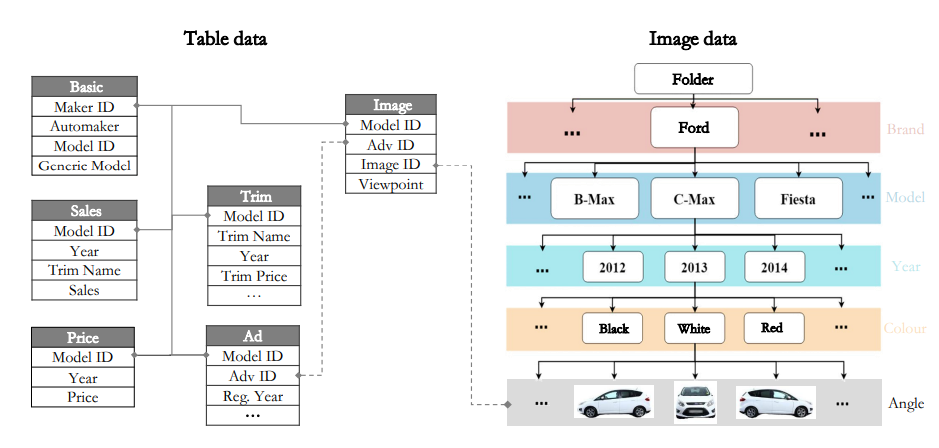
\includegraphics[width=0.9\textwidth]{general_data_tables.png}
    \caption{DVM-Car Dataset}
    \label{table:DVM-Car Dataset}
\end{figure}
\FloatBarrier


\noindent The \textit{Table data} part contains five CSV table. One of these table allows the access to images thanks to an URL that we can build. The others contain different information (see Figure~\ref{table:List of tables}). 
Then, images data are stored in a ZIP file. 
All of these data are accessible in the website: \url{https://deepvisualmarketing.github.io/}

\FloatBarrier
\begin{figure}[ht]
    \centering
    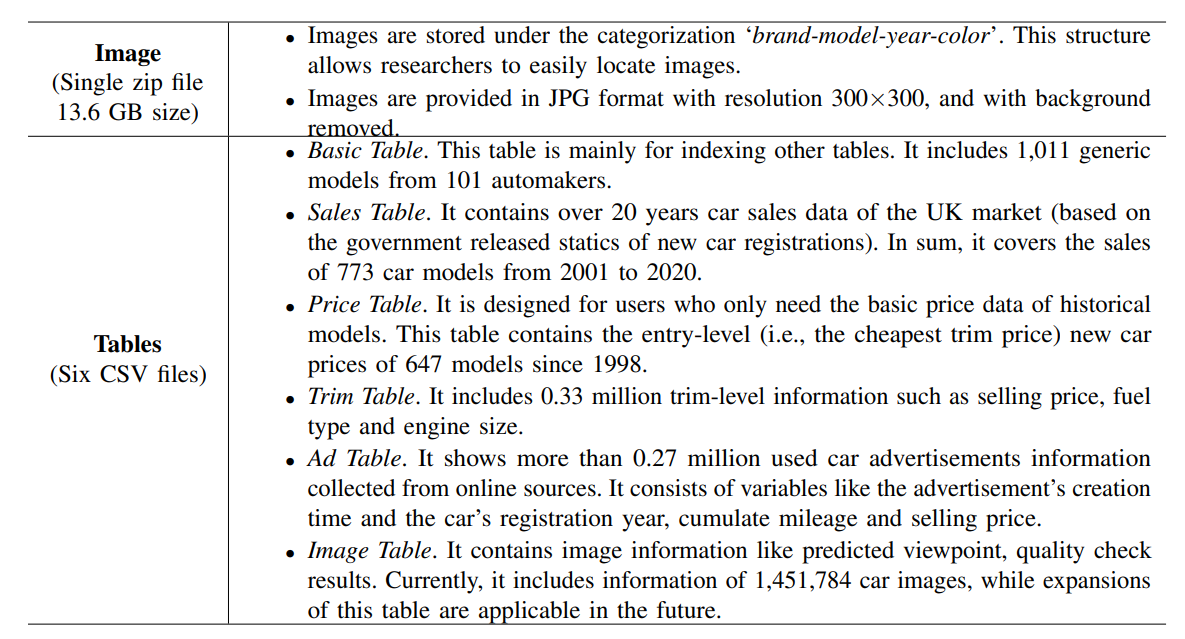
\includegraphics[width=0.9\textwidth]{overviewDVMdata.png}
    \caption{List of tables}
    \label{table:List of tables}
\end{figure}
\FloatBarrier

\noindent We decided to work with the tables \textit{Ad\_table} and \textit{Trim} for categorical and numerical data. For images we developed a class to access the images through a link build from the table \textit{Price} and \textit{Image}.
\noindent In the next two parts, we will explain our data choices and strategies. 


\subsubsection{Categorical and numerical data}

\paragraph{Data Description}
~~\\ [0.1 cm]

\noindent In order to create a dataset containing the numerical and categorical data, we have merged two tables:  \textit{Ad\_table} and \textit{Trim}.\\

\noindent The first table, \textit{Ad\_table} includes 268,255 observations and 24 variables. These variables describe the characteristics of vehicles such as \textit{size, color, price, model}, etc. These data can be categorical, such as the \textit{car manufacturer, model,} or \textit{gearbox type}. There are also numerical data such as \textit{engine power} and \textit{price}. Many missing data are present in this table, especially in the columns \textit{colors, annual tax, average mpg}, or \textit{top speed}. We will explain in the next section, named preprocessing, how we handled these missing data. Additionally, outliers have been identified in this table, which may be due to poorly entered data or the presence of unique car models very different from others. These anomalies will be thoroughly examined in the preprocessing of the data.\\

\noindent The second table called \textit{Trim} consists of 335,562 observations and 9 variables. A trim refers to a particular reference of a car model. We merged this table to the previous one to add the data \textit{gas\_emission} of the cars.\\

\noindent Following the merging of these two tables, we obtained a final table of 213K observations before the preprocessing. The objective of our work is to predict the price of cars, and thus our dependent variable is the \textit{Price} variable.\\

\noindent The table~\ref{variables} is the dictionary of variables that we have selected for our final dataset.\\

\begin{table}[ht]
    \centering
    \caption{Dictionary of Variables}
    \label{variables}
    \begin{tabularx}{\textwidth}{lclX}
        \toprule
        \textbf{Variable} & \textbf{Type} & \textbf{Description} \\
        \midrule
        Price & Float & Vehicle price. \\
        Runned\_Miles & Float & Miles traveled by the vehicle. \\
        Engin\_size & Float & Vehicle engine size. \\
        Engine\_power & Float & Vehicle engine power. \\
        Wheelbase & Float & Vehicle wheelbase. \\
        Height & Float & Vehicle height. \\
        Width & Float & Vehicle width. \\
        Length & Float & Vehicle length. \\
        Average\_mpg & Float & Average fuel consumption in miles per gallon. \\
        Gas\_emission & Float & Vehicle gas emission. \\
        Top\_speed & Float & Vehicle maximum speed. \\
        Seat\_num & Int & Number of seats in the vehicle. \\
        Door\_num & Int & Number of doors of the vehicle. \\
        Body\_type & String & Vehicle type. \\
        Gear\_box & String & Gearbox type. \\
        Fuel\_type & String & Fuel type. \\
        \bottomrule
    \end{tabularx}
\end{table} 

\paragraph{Preprocessing} 
~~\\
\noindent Before turning to our predictive analysis, it was necessary to preprocess our data such that it can be feed to different models.\\

\noindent In order to carry out preprocessing in a uniform and structured way, we have opted to use object-oriented programming (OOP). This is a method of creating classes to create and manipulate objects, in this case observations. This class, called \textit{preprocess\_Ad\_Table\_Trim}, enabled efficient and optimized preprocessing. First, we renamed the columns of the merged table to have standardized column names so as to have the same structure for all variables. Then, after an analysis of the missing values, we decided to delete them, considering our already very large and complete database. For some variables, such as \textit{average mpg, engine size, engine power} and \textit{top speed}, we decided to impute the missing values by the specific average for each type of model. We made this choice because there were many missing values in these variables, which we perceived as very important in our database. \\

\noindent Next, we converted all categorical data into numerical format using the \textit{one\_hot\_encoding} function, which creates binary variables, making it easier to integrate this information into machine learning models. However, this method tends to create a lot of features and this transformation is not needed for all categorical data. Therefore, we decided to encode with the one-hot-encoder the variables \textit{Body\_type, Gear\_box, Fuel\_type} but not \textit{Door\_num} and \textit{Seat\_num}. These last two were transformed as two columns, containing as many unique values as the possible number of doors or seats.

\noindent After identifying outliers, we removed the 1\% highest prices and data with zscores greater than 4. The z-score method, also known as standard-score is a statistical for standardization that measures and quantifies the relationship of a data point with the mean of a group of data points, in other words how far from the mean a data point is. The formula is : \[Z = \frac{{X - \mu}}{{\sigma}}\] It assigns a high score to values that appear to be outliers. This step led to the removal of around 10K observations, representing x\% of our initial database. (see for the number of NaN's deleted).\\

\noindent Finally, the last step was the standardization, performing with the formula explained previously. It is an essential step in machine learning to rescale the values. It allows us to have data on a common scale, making them comparable. We decided to choose standardization over normalization because it is recommended for algorithms like K Nearest Neighbors, where scale sensitivity is very important. Thanks to the creation of this automated class, we obtain a class that ensures the creation of a coherent data set, ready to feed machine learning models. \\



\subsubsection{Image Data}

\paragraph{Data Description}
~~\\ [0.1 cm]

\noindent The ZIP file contains 1,451,784 car images. They have already been reworked by the creators of the database. The backgrounds are all white, the images are well refocused, and above all, the positions of the cars have been predicted (see Figure~\ref{table:images without transformations}). This prediction is available in the \textit{Image} table. This is an important information because we will start by predicting the prices of cars with a front-view photo, otherwise with all the possible views, the task might be too complex for the model to learn.\\

\noindent As our first idea was to concatenate two models, taking the last layer of a CNN model, we had to link each image to its price from the \textit{Ad\_table}. Unfortunately, we realised during the processing part that we were losing a lot of images. Even though there might have a solution, we struggled with the code and decided to change our strategy. We then decided to link images to prices through the \textit{Price} table. It contains entry prices of 647 models from the last two decades. 
As we might have different photos of the same model, we then duplicated and assigned those 647 prices to many images. Therefore, we attributed a price to each data of \textit{Image} table when the \textit{Maker, Genmodel, Genmodel\_ID} and \textit{Year} were the same.\\

\noindent Then, we had a dataframe with a price and information to reach each image. To do so, we built the class DVMdataset (available in the library.py code). This class takes as input the \textit{Price} table merged to the \textit{Image} table, the directory of the unpacked folder with all the images, and a parameter for the transformation of the data. 
\noindent Here are the three methods our class is using: \\

\begin{itemize}
    \item \textit{unpack all images} : iterates data in our dataframe and will find the associated image by navigating through the folders of the ZIP file. Once this image is found (if it is), the price of the data is assigned to it.

    \item \textit{\_\_getitem\_\_} : returns an image with a certain transformation strategy, and with its index. It is a necessary element to use pytorch dataloaders, and it also allowed us to print our images in an easy way.
    
    \item \textit{\_\_len\_\_} : returns the number of images in our dataset.
\end{itemize}

\FloatBarrier
\begin{figure}[ht]
    \centering
    \label{table:images without transformations}
    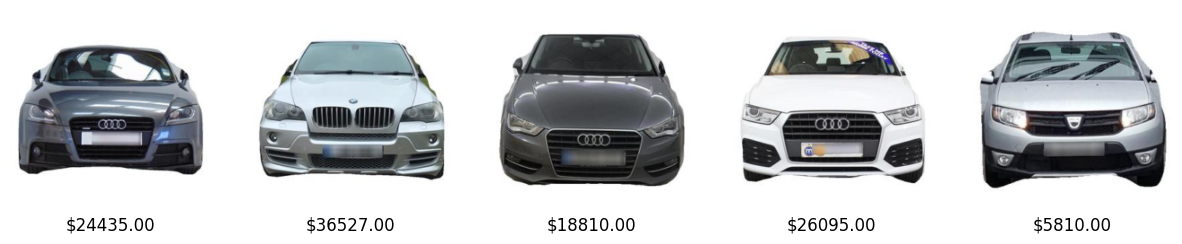
\includegraphics[width=1\textwidth]{images without transformations.png}
    \caption{Original images}
\end{figure}
\FloatBarrier

\subsubsection{Preprocessing and data augmentation}
The CNN model that we will use on our image data is a pre-trained model called Resnet18, which means that it is a model already optimized and trained. Therefore, before using this pre-trained model we had to normalize the data in the aim to have similar inputs. We used the means and the standard deviations in the Table~\ref{mean std} from the ImageNet dataset. This step makes the implementation of the images easier in RestNet18 and helps to obtain good results with the model. 

\begin{table}[h]
    \centering
    \begin{tabular}{cccc}
        \toprule
        & Red Channel & Green Channel & Blue Channel \\
        \midrule
        Mean & 0.485 & 0.456 & 0.406 \\
        Standard Deviation & 0.229 & 0.224 & 0.225 \\
        \bottomrule
        \label{mean std}
    \end{tabular}
    \caption{Mean and Standard Deviation Parameters}
\end{table}

\FloatBarrier
\begin{figure}[ht]
    \centering
    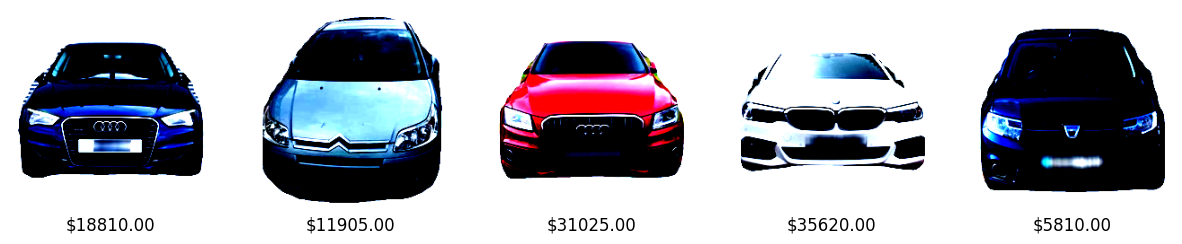
\includegraphics[width=1\textwidth]{testing images.png}
    \caption{Normalized images}
    \label{Normalized images}
\end{figure}
\FloatBarrier
 

\noindent As we had a dataset with a large amount of data, we decided to use data augmentation on the training set to train our model with different types of pictures. This step consists of taking the pictures from the original dataset and transform it with different operations. As we can see in Figure~\ref{training images}, we randomly rotated images from the initial pictures on the Figure~\ref{Normalized images}. Without any rotations, the model learns only from one precise point of view and will not be able to learn from a mistaken picture. 


\FloatBarrier
\begin{figure}[ht]
    \centering
    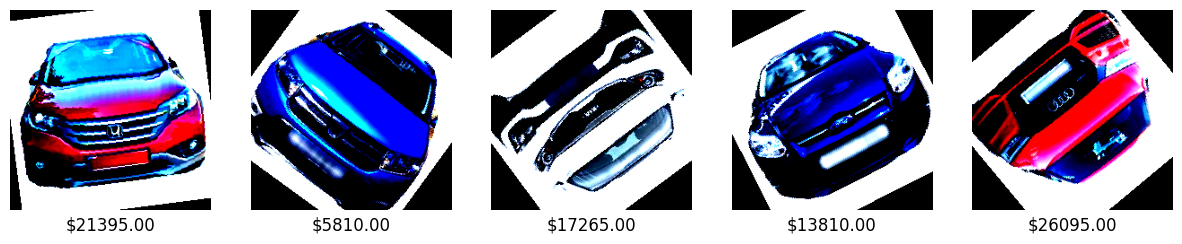
\includegraphics[width=1\textwidth]{training images.png}
    \caption{Rotated images}
    \label{training images}
\end{figure}
\FloatBarrier




\subsection{Machine Learning Algorithms and Methods}
Before turning to the results, this section will present our empirical strategy by introducing the machine learning algorithms and methods used. Put differently, we will explain and present our model selection by consulting academic literature as well as outline our approach and the python library used to estimate and tune these models.

Pr\subsubsection{K-Nearest-Neighbours (KNN)}
Since \cite{Samruddhi2020} proved to obtain promising results by fitting a KNN model for car price prediction, we decided to apply this approach to our dataset. Also it was an opportunity to have parametric and non-parametric models. \\

\noindent The K-Nearest Neighbors algorithm (KNN) is a supervised, non-parametric algorithm. In other words, it does not take a predefined function, but it is built on the data. It can be applied to classification or regression problems. The aim of this algorithm is to predict the value of an observation by averaging the values of the k nearest neighbors. Typically, the distance used for this algorithm is the Euclidean distance, which is \( d = \sqrt{{\sum_{i=1}^{n} (x_{2i} - x_{1i})^2}} \) in n-dimensional space, which measures the distance between two points in features space. The major challenge of this algorithm is to find the optimal $k$ that minimizes the error rate by taking into account the number of neighbors that can predict a value $\hat{y}$. The predicted $\hat{y}$ represents the average of these neighbors being the closest to the initial value to be predicted. In our case, to determine car prices, we will use the K Neighbors Regressor class from the scikit-learn package. 

\subsubsection{Extreme Gradient Boosting (XGBoost)}
First introduced by \cite{Chen2016}, the Extreme Gradient Boosting algorithm mainly gained popularity for its impressive performance in data science competitions. In general, XGBoost represents an extension of the Gradient Boosting algorithm proposed by \cite{Friedman2001} but comes with some additional advantages. Besides allowing for parallel computing and capabilities such as accounting for missing data, XGBoost offers more hyperparameters which  automatically account for overfitting. Although these advantages make the XGBoost a very powerful method it comes with some throwbacks. Due to its complexity, the XGBoost is considered a hardly to interpret black box model. However, since our task is mainly of predictive nature, the model's performance and its convenience are the main arguments for our choice. To fit the model on the categorical and numerical data only little preprocessing, i.e. category encoding, is required. Moreover, previous studies such as \cite{Gajera2021} have shown promising results using XGBoost to predict car prices. \\

\noindent Similar to Gradient Boosting, XGBoost fits a regression tree on so-called pseudo residuals calculated from previous prediction errors denoted by $\delta_{t} = y - \hat{y}_{t}$.\footnote{XGBoost starts from an initial prediction value $\hat{y}_{0}$ which by default is set to $0.5$ in the XGBoost library.} In contrast, however, XGBoost decides upon the best split by computing a measurement of similarity gain for each possible candidate split. This measurement quantifies the improvement in similarity of the pseudo residuals in each node after splitting the parent node into two child nodes. It includes a regularization parameter $\lambda$ scaling the similarity scores to control for nodes containing only few observations.\footnote{Otherwise, nodes with only few observations (pseudo residuals) would have misleadingly higher gain measures, indicating a good decision rule. Setting $\lambda > 0$ will reduce all gain measures inversely proportional to the number of observations per node.} The additional pruning parameter $\gamma$ denotes a minimum threshold in similarity gain to be exceeded by any binary split. If a potential split does not exceed this threshold it will not even be considered as candidate. At each iteration, the candidate split $(s, j)^{*}$ providing the best gain in similarity is chosen as decision rule for the $m^{th}$ branch in the tree. To make new predictions $\hat{y}_{t}$, the algorithm takes the initial prediction $\hat{y}_{0}$ and adds the predicted pseudo residuals of the previous iterations multiplied by a learning rate $\eta$.\footnote{The speed of convergence $\eta$ with range $[0,1]$ shrinks the added residual, and thus makes sure to converge slowly towards the original value $y$.} 
From this point, the algorithm repeats itself: The new prediction is used to compute the new pseudo residuals on which a new tree estimator will be fitted. The predicted residuals will be added to the sum of the initial prediction and the previous predicted residuals and so on. The procedure continues until a defined number of estimators is reached. \\

\noindent Thus, besides the common decision tree parameters such as maximum tree depth and minimum child weight, the challenge of tuning an XGBoost model is to find the optimal combination of the additional hyperparameters, namely the learning rate $\eta$, the number of estimators, regularization parameter $\lambda$, and pruning parameter $\gamma$. To do so, we make use of the GridSearchCV package from the scikit-learn library which finds the best model by fitting and comparing all possible models from a predefined set of parameter combinations using cross validation. An extensive grid search, however, requires to fit a vast number of models, and thus will be rather computationally inefficient. begin: First, we estimate an initial XGBoost to determine the optimum number of tree estimators for a given learning rate $\eta$, using cross validation.\footnote{These parameters must be tuned together, because to maintain a certain predictive power, reducing $\eta$ requires increasing the number of estimators and vice versa.} In a next step, we use the grid search to find the optimum tree structure, i.e. maximum tree depth and minimum observations per leaf. Having defined the general tree structure, we tune the pruning parameter $\gamma$ and search for the best regularization parameter $\lambda$.


\subsubsection{Multilayer Perceptron (MLP)}

\noindent Another interesting model to predict car prices is the multilayer perceptron model from the Neural networks family. 
\noindent Developed from the perceptron model (\cite{Rosenblatt1958}), the MLP introduces multiple layers of neurons, each capable of learning different aspects of the data and therefore permitting to capture complex relationships. As our categorical and numerical data are specific and their relationships and interactions might be various, building a MLP could model and capture some of these dynamics. The large DVM dataset containing a large amount of data, we should be able to train an accurate MLP model.\\

\noindent The first layer of the neural network contains as many neurons as features. It is from this layer that the data is introduce onto the Neural network. The flexibility of this model allows us to add as many layers with as many nodes as we want. In fact, those kind of parameters are called hyper-parameters and should be tuned with a grid search. The last layer size depends on the task at hand. As we want to predict prices, it is a regression task and therefore the last layer results in one node (for a classification task, we would set as many nodes as the number of classes). Another specificity of the MLP is that all neurons of a layer are connected to all neurons of the previous and following layers.
In between each layers, a linear transformation is applied to the data, and those linear transformations are plugged in an activation function. Those activation functions determine whether a node should be activated or not. It is where the non-linearities are captured, otherwise the model would not be able to capture complex relationships. To make the model learn, the backpropagation is a two-step process to update weights of the linear transformations. At first, in the forward pass, the data are passed in the network and compute the output. In the second part, the backward pass compute the gradient of the loss function with respect to each weights of the model. Then, this gradient is used to update the weights.\\

\noindent One of the main problem of neural networks is that we can quickly have a large number of weights and the model could end up overfitting. To avoid it, we can drop some neurons to neurons links with a certain probability. This method reduce the number of weights computing the output and being updated for a certain training step. 


\subsubsection{Convolutional Neural Network (CNN)}

\noindent As we explained in the introduction, some researchers such as Yang, S. Chen, and Chou (2018) used CNN on car images to predict the prices. Indeed, we will use a Convolutional Neural Network, which is part of deep learning that takes image data as inputs to train a model. We wanted to build our own model but it would take more time and lead to worse accuracy than a model that is already built. AlexNet and Resnet are two pretrained models well known for images tasks. AlexNet was developed by \cite{Krizhevsky2012} and was the first deep convolutional neural network applied to images. We decided to take Resnet18 introduced by \cite{Kaiming2016}, which is an amelioration of Alexnet. The particularity of this model is the residuality of the network, where the name comes from. The difference with the previous model is that the result does not only come from the output but also from the difference between the input and the output as we can see in Figure \ref{Resnet18}.

\noindent We opted for the ResNet18 model to maximize computational efficiency, given our limited computing resources. ResNet18 is chosen for its simplicity, consisting of only 18 layers.

\FloatBarrier
\begin{figure}[ht]
    \centering
    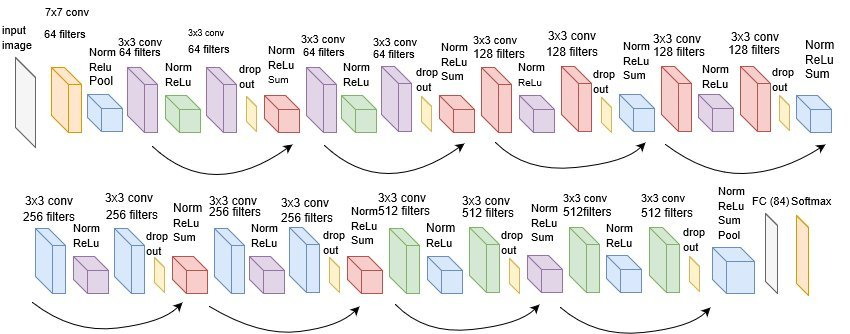
\includegraphics[width=0.85\textwidth]{resnet18.jpeg}
    \caption{Resnet-18 architecture}
    \label{Resnet18}
\end{figure}
\FloatBarrier

\noindent The Figure~\ref{Resnet18} explains the architecture of Resnet-18.
First, the Resnet model takes as inputs RGB images of size 224x224 pixels. The size of the images was adjusted in the preprocessing step. Thus, the first convolution composed of 64 filters also called kernel can be applied. This convolutional layer captures low-level features within the images. Subsequently, a batch normalization is performed, it is a step that corresponds in data normalization to scale the data and facilitate the machine learning processes. Following this, the model applies a first ReLU activation function to introduce non-linearity. The pooling step follows, acting as a reduction method as it reduces the size of the images. 
Will follow a sequence of four layers each containing two residual blocks, a total of 8 residual blocks.
Afterwards, the global average pooling is performed to obtain a single value that represents the average value of each pixel.  Then, we will reach the final output which is a single scalar value by using a fully connected layer, a linear regression which is the final layer of the Resnet model. In the context of a regression problem for price predictions, we delete the last step which the softmax activation function that computes probabilities to belong to a specific class in the classification problem, which is unnecessary for regression problems.\\



\subsubsection{Model-Agnostic Methods}
Since all of the applied machine learning methods are so-called black box algorithms, the results and individual feature effects on the target variable (car price) are hard to interpret. Model-Agnostic methods allow us to interpret such models by partially analyzing the effect of one feature on the outcome variable independent from the underlying algorithm. To generate the PDP, ICE plots, and SHAP values, we apply the SHAP python library on a smaller subsample. \\

\noindent \textbf{Partial Dependence Plots (PDP) and Individual Conditional Expectation (ICE)}\\
Introduced by \cite{Friedman2001}, the partial dependence plot (PDP) is a global model-agnostic method which isolates the marginal effect of an individual feature on the predicted target variable when fitting a machine learning model. \\

\noindent The method follows an experimental approach: For a given black box model, we examine the effect of a specific feature of interest \(x_S\) by artificially changing all of the feature's values in a systematic way and refit the model to obtain reference predictions while keeping all other features \(X_C\) fixed. More precisely, starting with the min(\(x_S\)), we change the feature's value of all observations to the very same occurrence until all values from the feature's set were once assigned and all reference predictive values were estimated. In a last step, we plot all the average of all these referential predictions against the feature's set of numbers, i.e. all possible values in the sample set the feature can take on.\footnote{This step makes the PDP a Monte Carlo experiment.} We obtain a step function displaying the marginal change in the target variable for the respective change in the feature's value while keeping all other feature's fixed (\cite{molnar2023}).\\

\noindent Putting aside the advantages, the PDP relies on the strong assumption that we have no correlations among the regressor variables. As to be shown in the exploratory analysis, our data violates this condition, and thus the PDP might not capture heterogeneous effects. To overcome this problem, we will make use of individual conditional expectation (ICE) plots. This \textit{local} model-agnostic method explains how the feature of interest affects the predicted value of an \textit{individual observation}. Put differently, the ICE decomposes the PDP (average marginal feature effect) into \textit{n} conditional relationships between each observation and its predicted value (\cite{goldstein2014}).\footnote{Vice versa, the PDP represents the average of the ICE curves.}  \\

\noindent \textbf{SHAP (Shapley Additive explanations)} \\
\noindent First introduced by \cite{lundberg2017unified}, SHAP is a model-agnostic method which is based on the game theoretically shapley values by \cite{shapely1953}. Shapley values investigate the contribution of each feature value to the prediction compared to the average prediction value. To do so, the main idea of shapley values is to translate the prediction task at hand into game theory. In game theory, players can form different coalitions to affect their payout. In this scenario, the prediction of an individual observation represents the game, the feature values of an observation are the players and the payout is the difference between the observation's actual prediction and the average prediction of all observations. To obtain a feature's contribution to the final prediction, we randomly draw a large number of observations for each of which we repeatedly, i.e. large number of times, draw a random feature value from the feature set. Averaging the differences in predictions of these artificially generated observations and their actual prediction values provides us the marginal feature's contribution for a given coalition of features. To obtain the shapley value of the feature of interest, we repeat this procedure for all possible coalitions, i.e. feature combinations, and compute the \textit{average} marginal contribution \cite{molnar2023}.\\

\noindent The game theoretical foundation of shapley values make them a solid and commonly used method to explain black box machine learning algorithms. For this reason, we will apply the SHAP python library as second model-agnostic method to interpret our trained models.


\subsubsection{Information Reduction Methods}\\

\noindent After encoding all categorical variables, we are facing a dataset of 33 features, and thus operate with high dimensional data. This might lead to problems when fitting a model which does not automatically regulates its complexity but tends to overfit. That said, as comparisons we will apply two approaches of information reduction and evaluate for improvement in model performance.\\

\noindent \textbf{Principle Component Analysis} \\
The Principal Component Analysis, also called PCA, is a reduction method developed by \cite{Pearson1901}. This reduction method consists of reducing the number of variables by creating a new set of variables called principal components, which are uncorrelated. These components are linear combinations of the original set of variables and their order corresponds to the component that captures the largest amount of variance. 
This method is useful to reduce significantly the number of variables while keeping an important portion of the information through the variance.\\


\noindent \textbf{Elastic Net}\\
\noindent As an alternative to information reduction methods, e.g. based on linear combinations of the feature variables such as PCA, penalized regression models can be applied for feature \textit{selection}. Especially when dealing with high dimensional data and highly correlated features, the elastic net represents a suitable regularized regression method. Proposed by \cite{Zou2005}, the elastic net outperforms the lasso regression by linearly combining its L1 regularization with the ridge L2 regularization. This way, the lasso's disadvantage of selecting only one variable from a correlated feature group is corrected.\\

\noindent Since our data shows strong collinearity among various features (see Figure \ref{Correlation matrix}) such as the car's dimensions (width, height, length, wheelbase) or among the engine specifications (engine size, engine power, gas emission, and top speed), the elastic net is a promising approach. This way, we ensure not to exclude good estimators that show collinearity. Against this background, the elastic net might help us to reduce the complexity of our black box models, and thus the risk of overfitting. More concretely, from the elastic net regression we can identify the most important features based on which we can refit our machine model. Effectively, we will have reduced the dimensions of the fitted data. \\

\noindent However, applied to the XGBoost model, this will probably not yield better model performance. As explained in section 2.2.2, by construction, XGBoost selects the most important features automatically by comparing their predictive power at each binary split. Accordingly, this might even lead to a decrease in performance. Nonetheless, we want to demonstrate as well as compare this approach and, additionally, use the elastic net results as benchmark of a sophisticated linear model, both for the price prediction as well as for the XGBoost agnostic results.\\


\section{Results}
The following subsection will present our empirical results. We start by providing the exploratory analysis, i.e. some descriptive statistics. This way, we gain a better understanding of our data which will help us to better interpret our predictive results and derive the limitations of our empirical analysis.

\subsection{Exploratory Analysis}
\subsubsection{Descriptive Statistics}
~~\\
\noindent Descriptive statistics give us a better overview of our database.\\

\noindent Table \ref{Descriptive_statistics} shows the main descriptive statistics for these variables, with the number of values, the mean, the standard deviation, the minimum, the maximum and the quartiles. This gives us an idea of the distribution of these variables.\\


\begin{table}[h]
    \centering
    \begin{tabular}{lrrrrrrr}
    \toprule
           & Price & Runned\_Miles & Engin\_size & Engine\_power & Height & Width & Length \\
    \midrule
     count & 200676 & 200676 & 200676 & 200676 & 200676 & 200676 & 200676 \\
     mean & 10589.9 & 52352.4 & 1.8085 & 137.959 & 1535.76 & 1885.63 & 4334.15 \\
     std & 9496.06 & 39580.4 & 0.600646 & 60.2528 & 116.157 & 149.073 & 402.895 \\
     min & 100 & 2 & 0.66 & 50 & 1112 & 1475 & 2727 \\
     25\% & 3995 & 18250 & 1.4 & 99 & 1460 & 1770 & 4052 \\
     50\% & 7950 & 46000 & 1.6 & 120 & 1495 & 1875 & 4344 \\
     75\% & 13799 & 80000 & 2 & 168 & 1615 & 2013 & 4644 \\
     max & 56750 & 222000 & 4.6 & 429 & 1951 & 2365 & 5970 \\
    \bottomrule
    \end{tabular}
\end{table}

\begin{table}[h]
    \centering
    \begin{tabular}{lrrrrrrr}
    \toprule
           & Average\_mpg & Top\_speed & Gas\_emission & Wheelbase & Seat\_num & Door\_num \\
    \midrule
     count & 200676 & 200676 & 200676 & 200676 & 200676 & 200676 \\
     mean & 51.9473 & 120.585 & 152.543 & 2636.89 & 4.92767 & 4.45066 \\
     std & 12.3794 & 15.6977 & 37.9909 & 169.992 & 0.790823 & 0.931608 \\
     min & 9.8 & 80 & 0 & 1445 & 1 & 2 \\
     25\% & 43.5 & 109 & 129.096 & 2511 & 5 & 4 \\
     50\% & 51.4 & 118 & 142.786 & 2634 & 5 & 5 \\
     75\% & 61.1608 & 130 & 167.316 & 2741 & 5 & 5 \\
     max & 134.5 & 189 & 440 & 4065 & 9 & 5 \\
    \bottomrule
    \end{tabular}
    \caption{ Descriptive statistics}
    \label{Descriptive_statistics}
\end{table}

\FloatBarrier

\noindent Interpretation: \textit{On average, a car costs \$10,589.90} \\

\noindent Figure~\ref{Boxplot prices} illustrates the distribution of our target variable, the price. This boxplot reveals a tight distribution, indicating that most data are concentrated between \$5,000 and \$10,000, with little dispersion. The median, represented by the central line of the box, lies at \$9,000, meaning that 50\% of the data are below this value. 
\noindent The whiskers on the graph, generally associated with extreme values, show points on the right-hand, to be identified as outliers. Despite efforts to clean up the price variable, reducing the range of values from \$100,000 to \$56,000, the graph shows the persistence of numerous outliers. By choice, we have decided to retain these values, considered less aberrant than those in our initial dataset.
\noindent This box plot shows an asymmetry in the distribution of our dependent variable.

\FloatBarrier
\begin{figure}[ht]
    \centering
    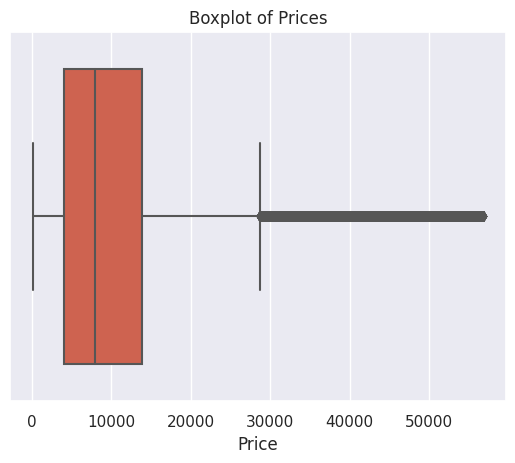
\includegraphics[width=0.28\textwidth]{boxplot price.png}
    \caption{Boxplot of prices}
    \label{Boxplot prices}
\end{figure}
\FloatBarrier

\noindent Next, Figure~\ref{Relationships} shows the relationship between each float variable and the price. Those graphs permit to detect outliers in the first instance, which we removed in the pre-processing step. It can also be interesting to study the distribution of prices for each variable, in order to familiarize ourselves with the dataset we will later use to train our models. Finally, this approach allows us to identify trends between the independent variables and the dependent variable, price. For example, we can observe a positive correlation between vehicle price and engine power.

\FloatBarrier
\begin{figure}[ht]
    \centering
    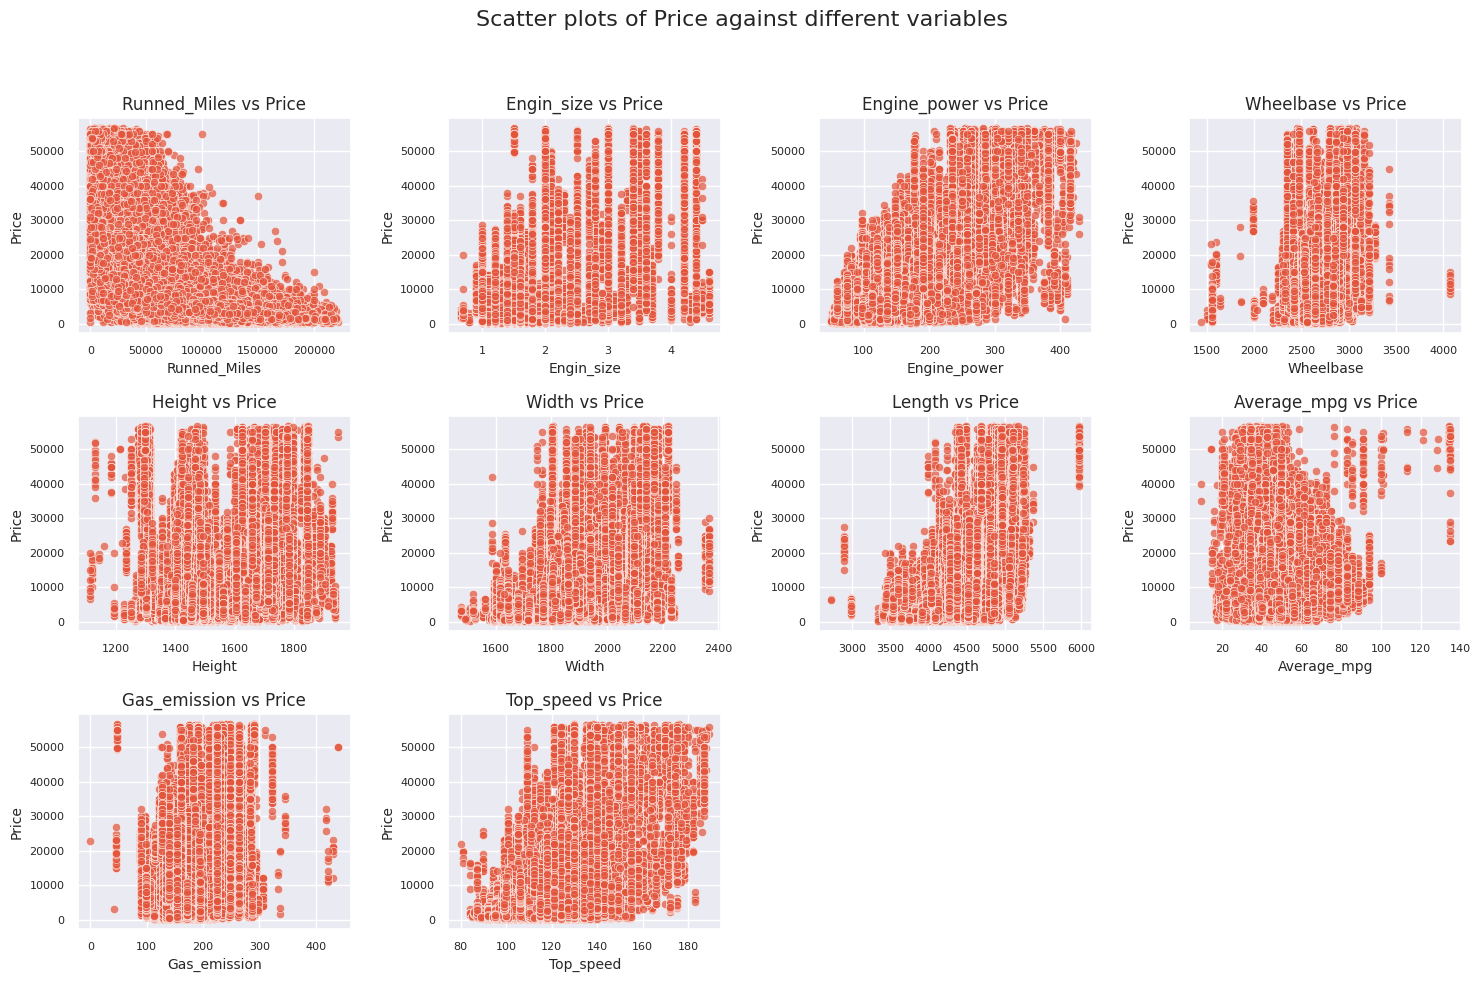
\includegraphics[width=0.8\textwidth]{numerique variables.png}
    \caption{Relationship between quantitative variables and the price}
    \label{Relationships}
\end{figure}
\\
\FloatBarrier

\noindent We chose to use boxplots to examine the relationship between car prices and two integer variables, to make the graphs more understandable. 
Figure~\ref{Two boxplots} illustrates the boxplots for the number of doors and the number of seats. 
After preprocessing, we found that there are only 4 possible values for the number of doors. Among these values, three-door cars seem less dispersed. Concerning the number of seats, an outlier persists with zero seats, probably due to an incorrect data entry. In addition, the data show very divergent behavior in terms of price depending on the number of seats. For example, models with 2, 5, 7 and 8 seats tend to have a lower price, never exceeding \$30,000 for these models.

\FloatBarrier
\begin{figure}[ht]
  \centering
  \begin{subfigure}{0.35\textwidth}
    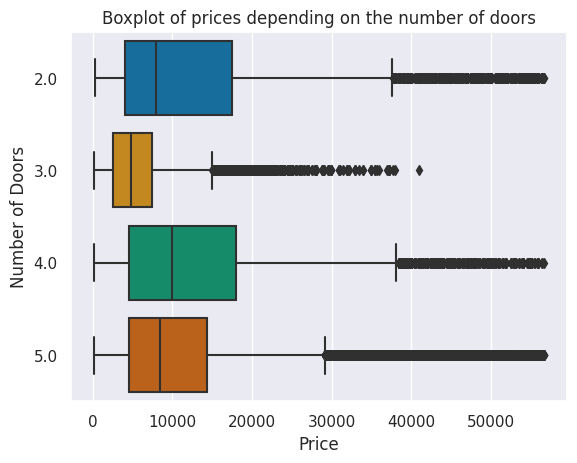
\includegraphics[width=\linewidth]{number of doors.png}
    \caption{Number of doors}
    \label{fig:image1}
  \end{subfigure}
  \begin{subfigure}{0.35\textwidth}
    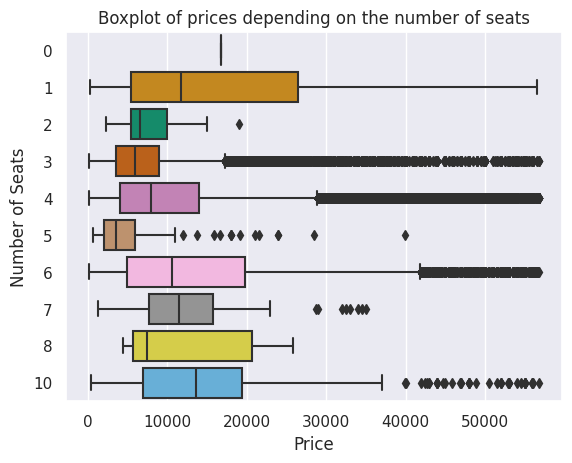
\includegraphics[width=\linewidth]{number of seats.png}
    \caption{Number of seats}
    \label{fig:image2}
  \end{subfigure}
  \caption{Boxplots of prices depending on integer variables}
  \label{Two boxplots}
\end{figure}
\FloatBarrier


\noindent Finally, to analyse the qualitative data, we also use boxplots (see Figure~\ref{Three boxplots}). The Figure on the left reveals the differences in the dispersion of the data according to the fuel type. The boxplots indicate significant variations between different fuel categories, highlighting the potential impact of this variable on vehicle price prediction. 
The middle boxplot, associated with vehicle types, shows a similar distribution for the first seven types, while the last two types \textit{Car Derived Van} and \textit{Limousine} stand out clearly from the others by tending towards lower prices, probably due to a low amount of observations. 
Finally, the last boxplot on the right shows a trend whereby cars with automatic gearboxes tend to be more expensive than those with manual gearboxes. 

\FloatBarrier
\begin{figure}[ht]
  \centering
  \begin{subfigure}{0.36\textwidth}
    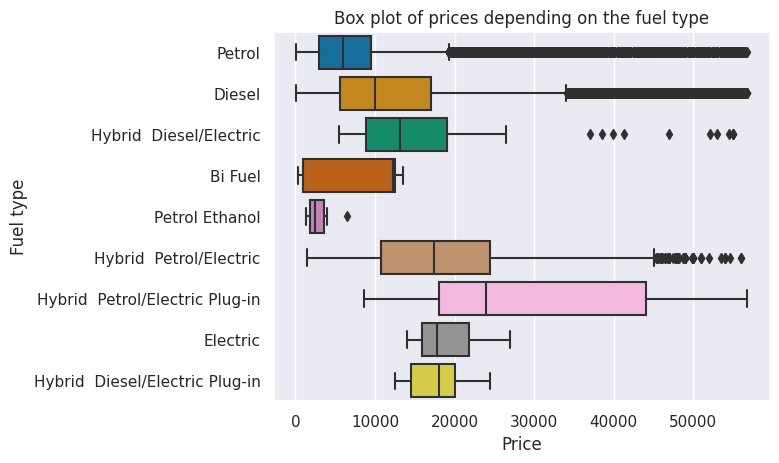
\includegraphics[width=\linewidth]{fuel type.png}
    \caption{Fuel type}
  \end{subfigure}
  \hfill
  \begin{subfigure}{0.32\textwidth}
    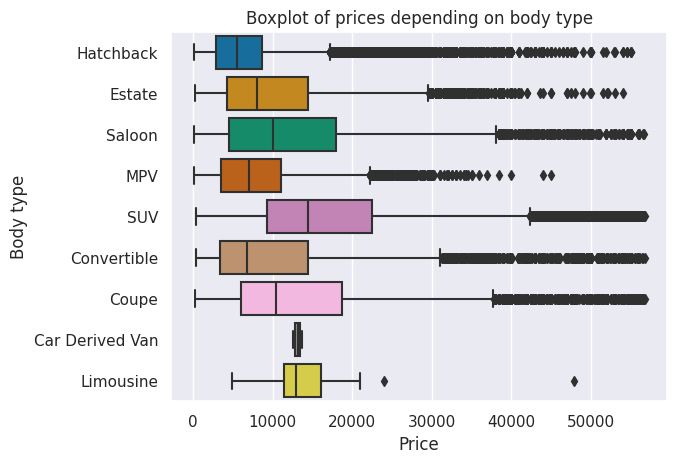
\includegraphics[width=\linewidth]{body type.png}
    \caption{Body type}
  \end{subfigure}
  \hfill
  \begin{subfigure}{0.30\textwidth}
    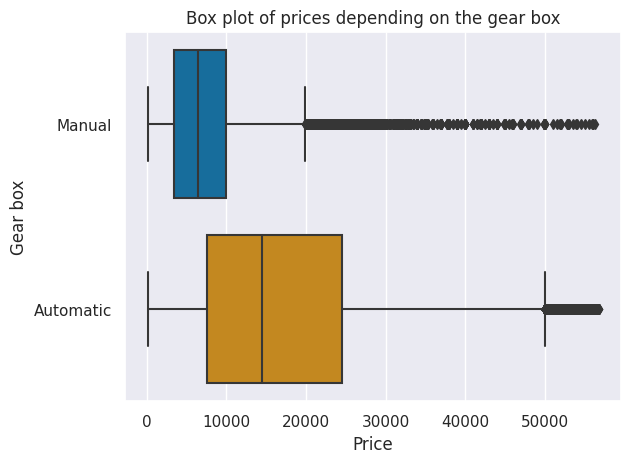
\includegraphics[width=\linewidth]{gear box.png}
    \caption{Gear box}
  \end{subfigure}
  \caption{Dependance between qualitative variables and the price}
  \label{Three boxplots}
\end{figure}
\FloatBarrier

\subsubsection{Correlation matrix}

\noindent The correlation matrix is important for understanding the correlations among features and summarize the dataset. Figure~\ref{Correlation matrix} shows an area where many features are correlated to each other. Some variables are highly correlated, such as \textit{length} and \textit{wheelbase} with a coefficient of 0.89. The large amount of values nearly equal to zero is due to the one-hot encoded variables which are vectors of zero and one. Since we had many different categories, those new features contain much more zeros than ones.

\FloatBarrier
\begin{figure}[ht]
    \centering
    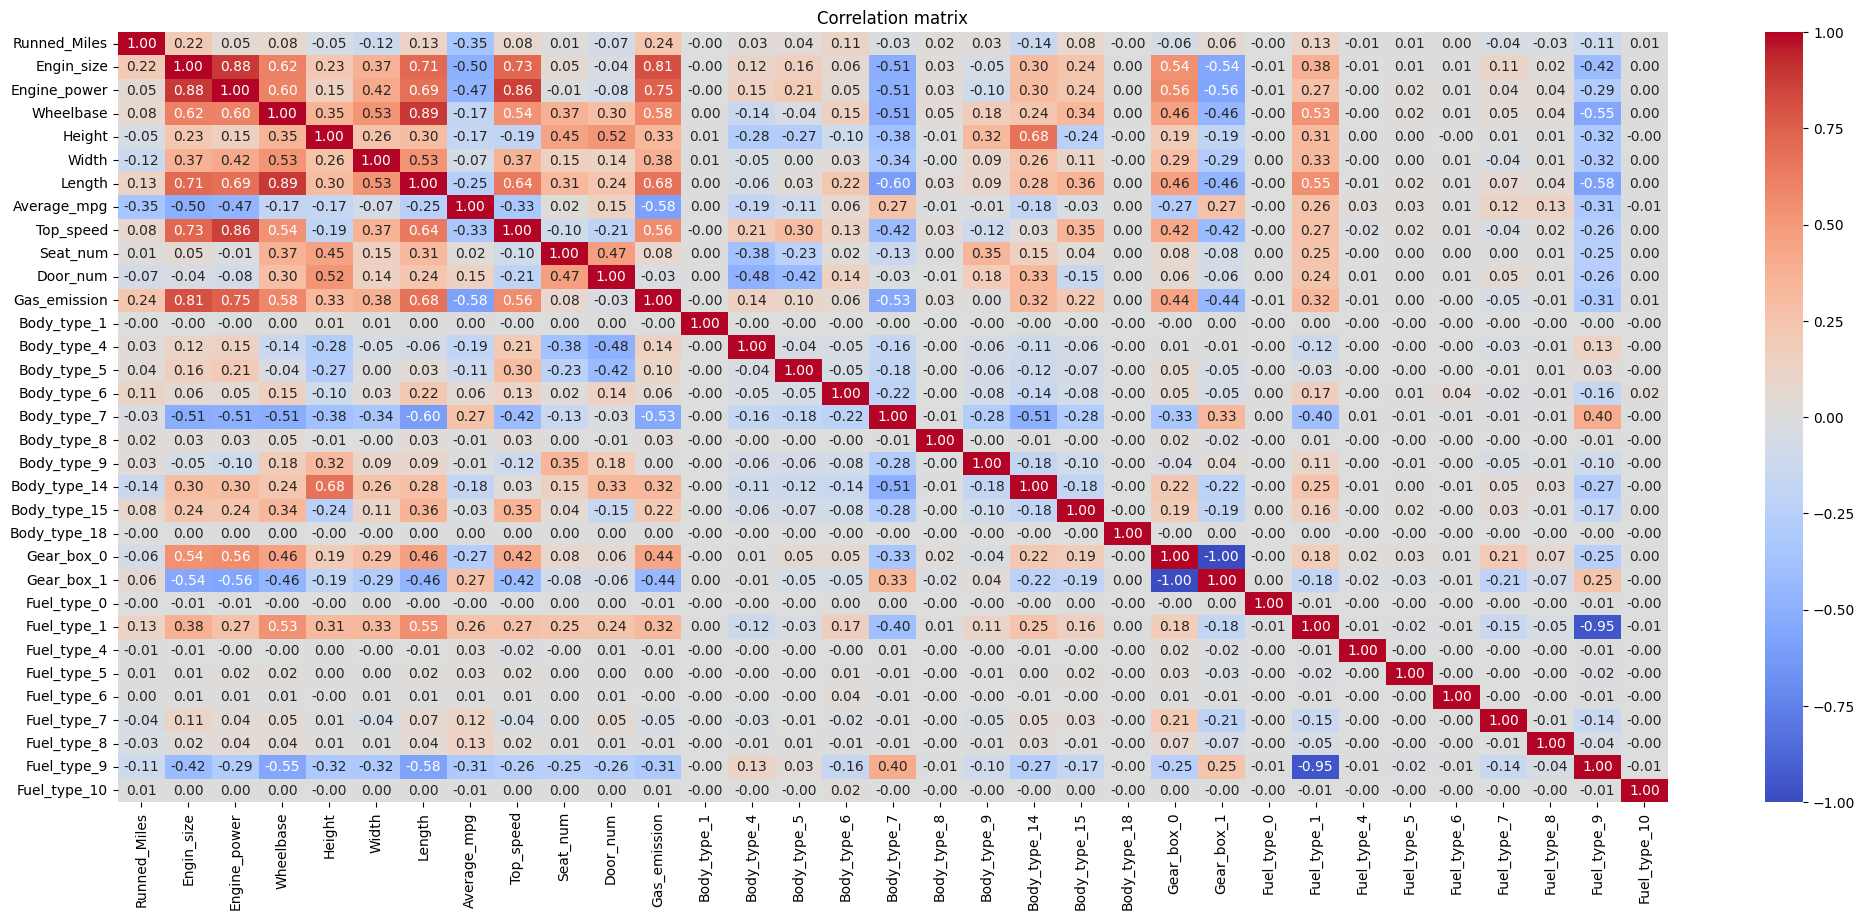
\includegraphics[width=0.90\textwidth]{Correlation matrix.png}
    \caption{Correlation matrix}
    \label{Correlation matrix}
\end{figure}\\
\FloatBarrier

\subsubsection{Price distribution of images}
\noindent Given that the prices and models that we have preprocessed are not exactly the same as for the previous part, we had to re-establish a choice of removing outliers. As we can see below, we have many outliers for cars above \$60,000. To keep a significant number of images and to complicate the tax on our CNN model, we decided not to keep images with an associated price greater than \$50,000 .

\begin{figure}[ht] 
    \centering

    \begin{subfigure}[b]{0.35\textwidth} 
        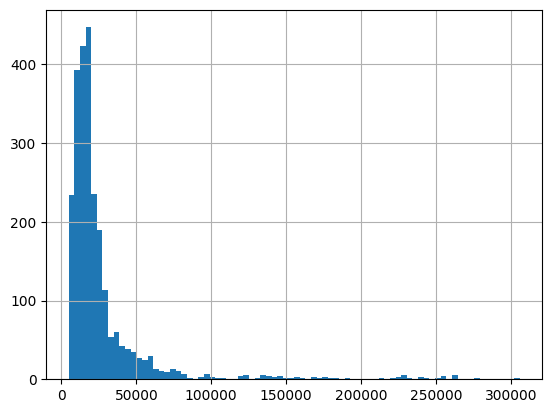
\includegraphics[width=\textwidth]{price_image_distribution_1.png}
        \caption{All images}
        \label{fig:image1}
    \end{subfigure}
    \begin{subfigure}[b]{0.35\textwidth}
        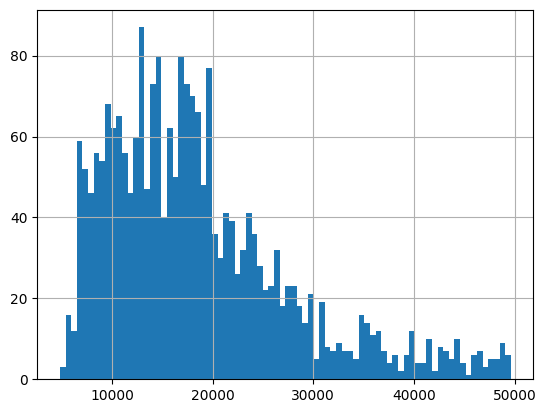
\includegraphics[width=\textwidth]{price_image_distribution_2.png}
        \caption{Without outliers}
        \label{fig:image2}
    \end{subfigure}

    \caption{Distribution of prices for front view images}
    \label{fig:Price distribution}
\end{figure}


\subsection{Predictive Analysis: Car price prediction with classical data}
For each of the above introduced machine learning models, this section will outline how the models were applied and fine tuned. Furthermore, we will exploit the chosen global and local model-agnostic methods to interpret our results in terms of feature effects and apply information reduction methods to these models.\\

\noindent To make the hyperparameter tuning as well as the model results more interpretable, we decided to evaluate the model performance using the root mean squared error as evaluation metric (RMSE). In contrast to other error metrics such as the mean squared or mean absolute error, the RMSE measures the error in the same unit as our target variable \textit{and} assigns much larger weights to larger errors.

\newpage

\subsubsection{K-Nearest Neighbors (KNN)}
\noindent \textbf{Model Tuning}\\
\noindent Initially, we started by optimizing k, representing the number of neighbors. To determine this hyperparameter, we trained the KNN model for each k ranking from 1 to 20. By comparing the RMSE of the train set and the validation set, we selected the value of this hyperparameter. As we can see in Figure~\ref{Optimal k}, the k minimizing the RMSE of the validation set with a score of 1667 is 4. 

\FloatBarrier
\begin{figure}[ht]
    \centering
    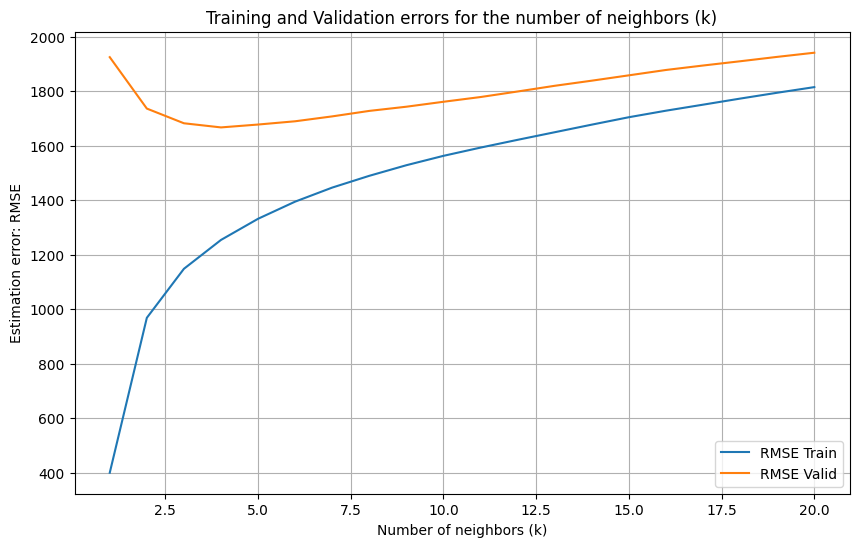
\includegraphics[width=0.45\textwidth]{Nb k.png}
    \caption{Training and Validation errors for the number of neighbors (k)}
    \label{Optimal k}
\end{figure}
\FloatBarrier

\noindent After selecting the best model, we applied it to our test set to see the score on unseen data. The Table~\ref{KNN results} summarizes the results of the different sets. The final score on the test set is 1719. 
Unfortunately, because KNN is a non-parametric model, we could not apply interpretable models, such as Shapley values, to explain the contribution of the variables to the final result and compare them with the Shapley values of the XGBoost model and the MLP model. Indeed, \cite{Molnar2022} explained that KNN is an instance-based learning algorithm, which can not be interpretable with a high number of features.

\FloatBarrier
\begin{table}[h]
    \centering
    \begin{tabular}{lccc}
        \toprule
        \multirow{\textbf{Set}} & \textbf{RMSE} \\
        & \textbf{(k=4)} \\
        \midrule
        \textbf{Training} & 1254.05 \\
        \textbf{Validation} & 1667.01 \\
        \textbf{Test} & 1719.35 \\
        \bottomrule
    \end{tabular}
    \caption{KNN Model Results with k=4}
    \label{KNN results}
\end{table}
\FloatBarrier

\noindent \textbf{Principle Component Analysis}\\
\noindent In order to improve the performance of the model and avoid overfitting we thought about reducing the features of the train set. As we observe in the data description part, some variables are highly correlated. 
To reduce the dimensions of our model, we chose the Partial Component Analysis method. This is an approach that reduces the dimensions of a dataset while preserving the variance of the initial data. The initial database, expressed in a high-dimensional space, will be reduced to a lower-dimensional space, which will be the space of the selected principal components. 

\noindent In order to choose the optimal number of dimensions, we can visualize the variance explained by each component (see Figure~\ref{PCA}). With the aim of 95\% of the variance explained by our new dataset, we decided to select the first 11 components. Thus, we reduced our dataset from 33 variables to 11 principal components. 

\FloatBarrier
\begin{figure}[ht]
    \centering
    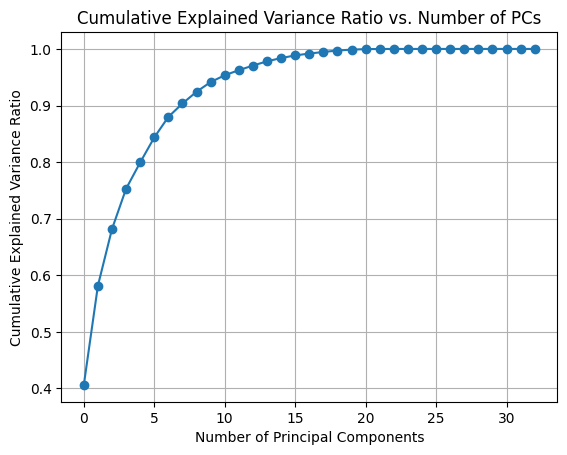
\includegraphics[width=0.45\textwidth]{PCA.png}
    \caption{Training and Validation errors for the number of neighbors (k)}
    \label{PCA}
\end{figure}
\FloatBarrier

\noindent Finally, we trained the KNN model on the PCA-transformed training set and evaluated its performance on the test set.
This enabled us to save processing time without degrading the results obtained, which are similar to the test results with the set of variables as we can see in Table~\ref{KNN results PCA}.

\FloatBarrier
\begin{table}[h]
    \centering
    \caption{KNN Model Results with k=4 and PCA=11}
    \begin{tabular}{lccc}
        \toprule
        \multirow{\textbf{Set}} & \textbf{RMSE} \\
        & \textbf{(k=4 and PCA=11)} \\
        \midrule
        \textbf{Training} & 1272.46 \\
        \textbf{Test} & 1735.86 \\
        \bottomrule
    \end{tabular}

    \label{KNN results PCA}
\end{table}
\FloatBarrier


\subsubsection{Extreme Gradient Boosting (XGBoost)}
As described in section 2.2.2, we follow a step-by-step approach to train and tune our XGBoost model. For our baseline XGBoost, we set $\eta = 0.1$, $max \; tree \; depth = 8$, $min\; child \; weigth = 1$, $\gamma = 0.1$, and $\lambda = 1$ and let the regressor fit as many trees until the next 500 additional estimators do not significantly improve the validation error.\footnote{These values are either standard values of the XGBoost libraray or are common used values for baseline models.} The grey line in Figure \ref{xgb_num_estimators} indicates that for the given learning rate, the optimum number of estimators is 765.

\begin{figure}[ht]
    \centering
    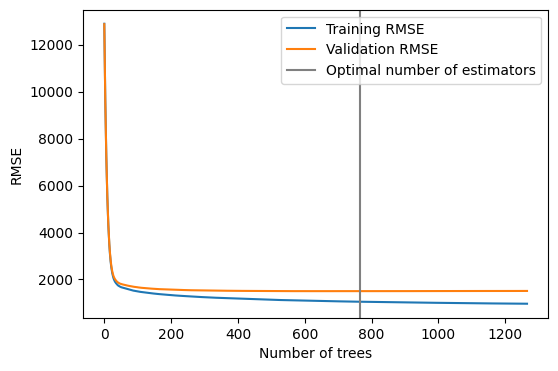
\includegraphics[width=0.5\textwidth]{xgb_num_estimators.png}
    \caption{Training and validation RMSE for different number of estimators with $\eta = 0.1$}
    \label{xgb_num_estimators}
\end{figure}
\FloatBarrier

\noindent The baseline XGBoost shows a RMSE of 1,454.62 and an $R^{2}$ of 0.9768. Thus, the default hyperparameter specifications already provide very good predictions which is in line with the overall high performance of the XGBoost algorithm.\\

\noindent \textbf{Model tuning} \\
\noindent In a first tuning step, we aim to find the optimal tree depth and child weight. Our grid search results outperform the baseline XGBoost with an RMSE of 1,432.99 ($R^{2}$ of 0.9977) when setting $max \; tree \; depth = 7$ and $min\; child \; weigth = 1$. Second, we find that setting $\gamma = 0$ neither improves nor worsens our model performance. This is surprising since the child weight is set to the minimum value of 1, and thus model overfitting should be expected. One explanation might be that the maximum tree depth as well as the number of estimators already regulate the model complexity sufficiently. Third, by setting the subsample size parameter from our baseline 0.8 to 1, our model improves by approx. 8 points in terms of RMSE.\footnote{This tuning step was not introduced in our empirical strategy (section 2.2.2) but represents another optional parameter which determines the size of the sample on which a new tree estimator is fitted.} And in a fourth and last step, increasing the regularization parameter lambda to 1.5 yields a slightly improved model performance with an RMSE of 1,418.60 and explains 97.79\% ($R^{2}$) of our data. Figure \ref{performance_evaluation} visualize the evaluation of the model performance by tuning step.

\begin{figure}[ht]
    \centering
    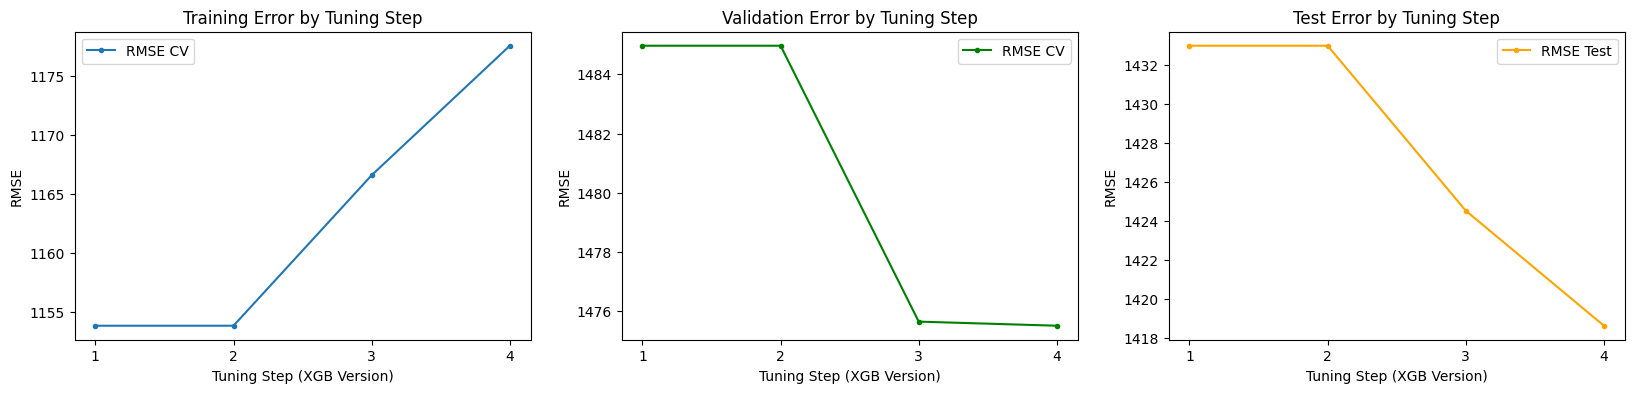
\includegraphics[width=0.9\textwidth]{rmse_evaluation.png}
    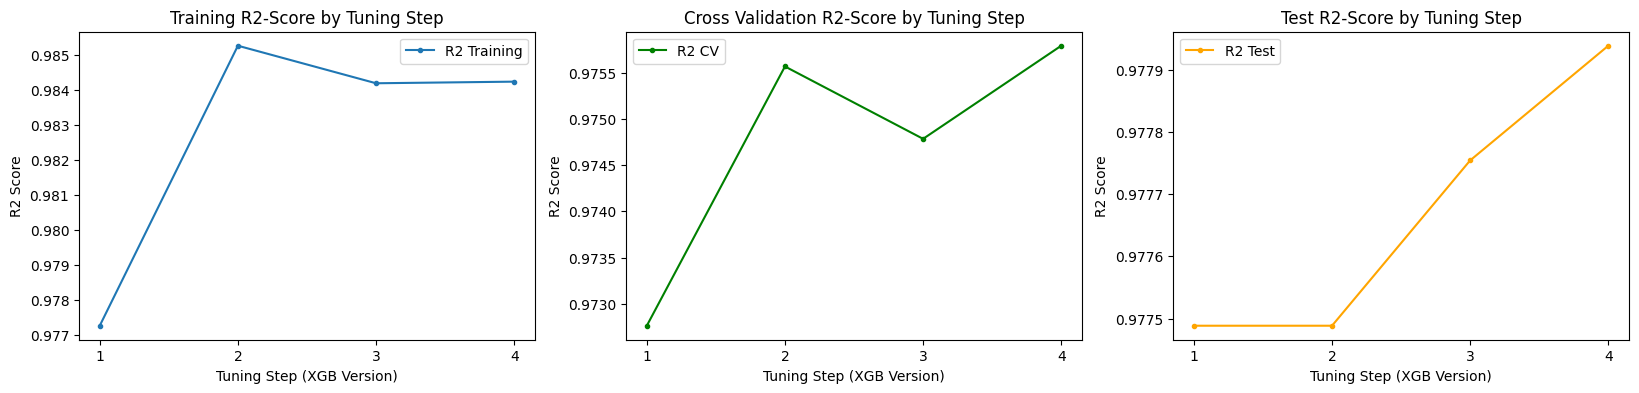
\includegraphics[width=0.9\textwidth]{r2_evaluation.png}
    \caption{Evaluation of RMSE and $R^2$ scores by tuning step}
    \label{performance_evaluation}
\end{figure}
\FloatBarrier

\noindent Even though the parameter tuning led to better model results, the average prediction error declined only by approx. \$36 compared to our baseline model. Put differently, the baseline model seems already to provide a very good model fit. The average error of approx. \$1,450 might be perceived as imprecise but will probably be different for different car price categories. That said, it might be interesting for further empirical studies to train specific car price prediction models for different car price categories. Figure \ref{xgboostbest} summarizes the model performance for the different sample sets.\\

\FloatBarrier
\begin{table}[h!]
    \centering
    \caption{Best XGBoost model performance}
    \begin{tabular}{>{\raggedright}p{5cm}rrr}
    \toprule
    \textbf{Set} & \textbf{RMSE} \\
    \midrule
    \textbf{Training} & 1178.93\\     
    \textbf{Validation} & 1475.50 \\
    \textbf{Test} &  1418.60 \\
    \bottomrule
     \label{xgboostbest}
    \end{tabular}
\end{table}
\FloatBarrier

\noindent \textbf{Individual Conditional Expectation Plots (ICE)} \\
To interpret the feature effects of our black box XGBoost, we must exploit post hoc model-agnostic. Moreover, we know that some methods cannot be applied due to correlations between some of our variables such as engine size, engine power, gas emissions and top speed are correlated. As explained in section 2.2.2 one possible approach is to produce ICE curves for our features of interest. Figure \ref{ice_plots} exemplary displays these plots for four of our explanatory variables.\footnote{Here, we present plots showing the most interesting effects. The remaining plots can be found in the attached notebook.} The thin lines represent the marginal feature effect of one observation on the car price and the thick blue lines represents the average feature effect, i.e. the PDP. The dotted grey lines mark the expected values, i.e.  average values, for the plotted variable (x-axis) and the price prediction (y-axis).\\

\noindent The ICE curves of plot (a) reveal a consistent negative effect of a car's mileage on its predicted price. For cars that have been driven more than 5,000 miles, the mileage leads to a prediction lower than the average XGBoost car price prediction. For the engine power in plot (b), we can observe the exact opposite, i.e. the more horsepower a car has, the higher its predicted price. Thus, both mileage and engine power are important variables for precise XGBoost predictions. For the car length in plot (c), we can observe that for cars longer than 4,000 and shorter than 5,200 units the length has a positive impact on the car price. Any car exceeding this threshold are not assigned a higher price due to its length. Interestingly, plot (d) indicates that a car's top speed has only a very limited impact on the predicted price, namely for very high top speed values. By design of the plots, it would be wrong to conclude that faster cars are not more expensive.The PDP and ICE curves are based on the XGBoost predictions, and thus based on those features (candidate splits) providing the best decision rules. Even though top speed is fairly correlated with a cars price (see Figure \ref{ice_plots}), the feature importance in terms of average added similarity gain\footnote{The variable importance plot can be found in the attached notebook} reveals that our XGBoost model relies very little on top speed. Put differently, our XGBoost model does not exploit the positive effect of top speed on a cars price which is captured by the relatively flat ICE plots. Yet, for all our features, the ICE curves follow the same trajectory, indicating that the PDP average explains the model predictions sufficiently well. \\

\FloatBarrier
\begin{figure}[h]
  \centering
  \begin{subfigure}{0.32\textwidth}
    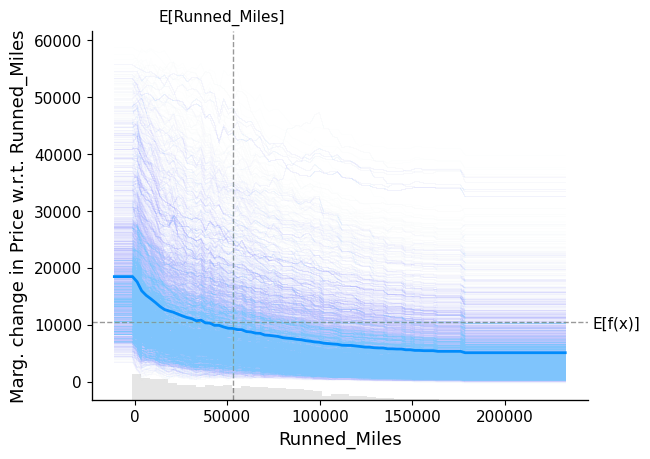
\includegraphics[width=\linewidth]{ice_runnedmiles.png}
    \caption{ICE Plots for Mileage}
    \label{ice_runnedmiles}
  \end{subfigure}
  \medskip
    \begin{subfigure}{0.32\textwidth}
    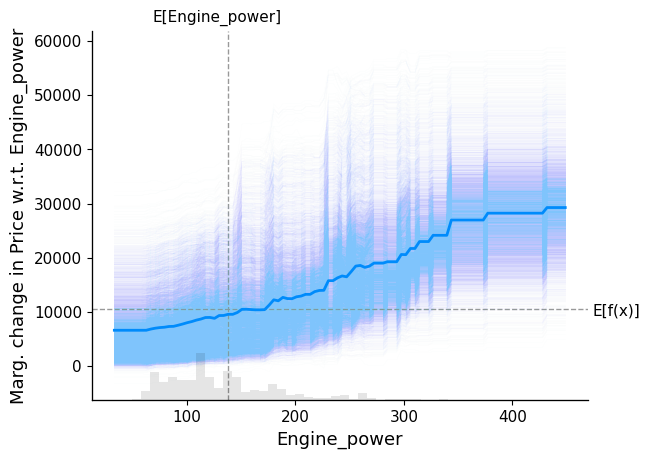
\includegraphics[width=\linewidth]{ice_enginepower.png}
    \caption{ICE Plots for Engine Power}
    \label{ice_enginepower}
  \end{subfigure}
  \medskip
  \begin{subfigure}{0.32\textwidth}
    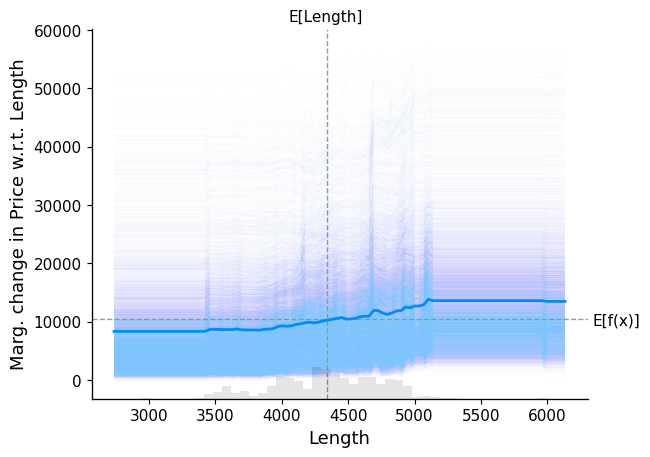
\includegraphics[width=\linewidth]{ice_length.png}
    \caption{ICE Plots for Length}
    \label{ice_length}
  \end{subfigure}
  \medskip
  \begin{subfigure}{0.32\textwidth}
    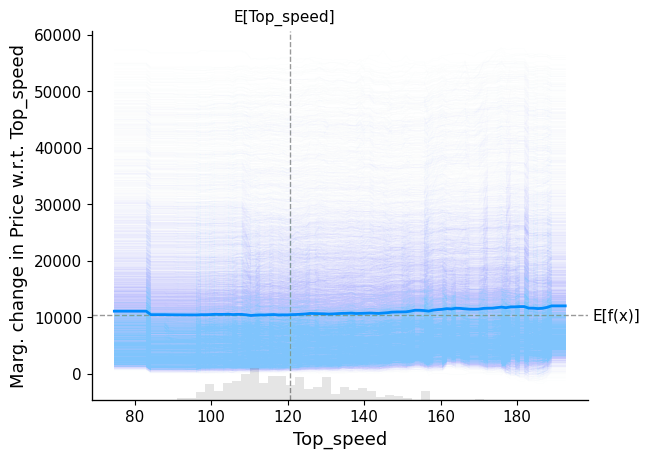
\includegraphics[width=\linewidth]{ice_topspeed.png}
    \caption{ICE Plots for Top Speed}
    \label{ice_topspeed}
  \end{subfigure}
  \caption{Independent Conditional Expectation Plots}
  \label{ice_plots}
\end{figure}
\FloatBarrier
\newpage
\noindent \textbf{Shapley Values} \\

Figure \ref{xgboostshapley} shows a beeswarm chart of shapely values supporting our discussion on the ICE plots. The mileage and engine power of a car have the biggest impact on the XGBoost predictions. This can be seen by the wide range and, even more importantly, by the many observations (dots) allocated to these two features. Low values for a car's mileage (engine power) lead to higher (lower) predicted prices which is indicated by the blue dots. Vice versa, high mileage (engine power) reduce (increase) the prediction in car prices. Moreover, we can see that the car dimensions, i.e. height, width, and length, have a moderate impact on the predicted price. The beeswarm graph for top speed is in line with our previous interpretation. To predict car prices, XGBoost exploits this feature only for few observations with high values. Furthermore, the clear separation between high an low values for some categorical variables such as fuel type 9 or gear box 0 are precise indicators to differentiate between low- and high-priced cars. 

\FloatBarrier
\begin{figure}[ht]
    \centering
    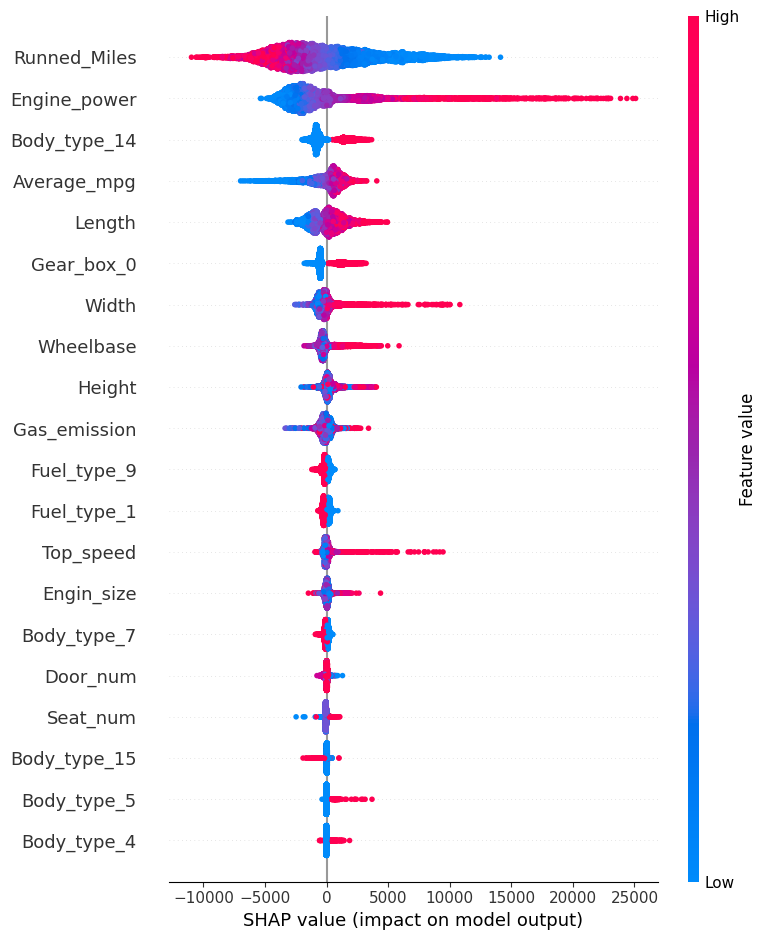
\includegraphics[width=0.5\textwidth]{xgboostshapely.png}
    \caption{Beeswarm shapley graph of XGBoost predictions}
    \label{xgboostshapley}
\end{figure}
\FloatBarrier

\noindent \textbf{Information reduction based on elastic net results} \\

\noindent To estimate an elastic net regression on our data with 33 features, some of which show collinearity, we first follow a grid search approach to find the best hyperparameters. Using a four-fold cross validation on 100 candidates, resulting in 400 fits, suggests to set $\lambda_{1} = 0.9$ and $\lambda_{2} = 0.1$. As expected, with an RMSE of 4497.61 and an $R^2$ score of 0.7782, we obtain worse results compared to our nonlinear competitors, i.e. KNN and XGBoost. These relatively poor results can most likely be explained with the lack in linear relationships between the features and the target variable. Regarding our motivation of feature selection, the elastic net coefficients suggest to drop 16 features, among others  height, top speed, seat number, and dummy variables for different body and fuel types.\footnote{The threshold for the coefficient to drop variables, was roughly determined by comparing the coefficient values. Find more detailes in the attached notebook.}\\

\noindent Fitting our XGBoost model on this new sample data yields an RMSE of 1443.99 and $R^{2}$ score of 0.9771, and thus slightly worse performance than our baseline XGBoost. These very similar results are not surprising. The ICE plots and shapely values have shown that for its predictions, the XGBoost mainly relies on mileage, engine power, body type average mpg and further variables which were not excluded from the elastic net variable selection. Table \ref{xgboostelastic} summarizes the performance of the XGBoost model fitted on 17 features selected by the elastic net.

\begin{table}[h!]
    \centering
    \caption{XGBoost model performance after dimension reduction (17 features)}
    \begin{tabular}{>{\raggedright}p{5cm}rrr}
    \toprule
    \textbf{Set} & \textbf{RMSE} \\
    \midrule
    \textbf{Training} & 1185.53 \\     
    \textbf{Validation} & 1499.47 \\
    \textbf{Test} &  1443.99 \\
    \bottomrule
     \label{xgboostelastic}
    \end{tabular}
\end{table}


\subsubsection{Multilayer Perceptron model (MLP)}

\noindent \textbf{Tuning the neural network} \\
\noindent To tune our hyperparameters, we have decided to focus on five parameters and swap them using the library \textit{Weights and Biases} (also known as \textit{Wandb}) : the \textit{dropout probabilities}, the \textit{activation function}, the \textit{batch size}, the \textit{learning rate} and the \textit{number of epoch}. In fact, the best number of epochs has been re-selected while training our best model during the cross validation.

\noindent For some hyperparameters, we set them up with a minimum and maximum value. During the run, \textit{Wandb} swap these parameters by taking a random number between bounds, following a certain distribution function. For other parameters, we chosen to set up some set of values. In this configuration, \textit{Wandb} does not draw a random value between two bounds, but a random value between different limited choices.


\begin{table}[h]
    \centering
    \caption{Parameters swapped through a distribution function}
    \label{table:Parameters swapped through a distribution function}
    \begin{tabular}{lrrrrrrr}
    \toprule
           & Minimum & Maximum & Distribution \\
    \midrule
     Learning rate & 0.0005 & 0.07 & Uniform  \\
     Batch size & 30 & 200 & Q\_log\_Uniform  \\
     Epoch & 3 & 15 & Q\_log\_Uniform  \\
    \bottomrule
    \end{tabular}
\end{table}
\FloatBarrier

\begin{table}[h]
    \centering
    \caption{Parameters swapped with limited sets}
    \label{table:Parameters swapped with limited sets}

    \begin{tabular}{lrrrrrrr}
    \toprule
           & Set of possible values \\
    \midrule
     Activation function & \begin{tabular}[c]{@{}l@{}}Tanh\\ Sigmoid\\ Relu\end{tabular} \\
     Dropout probabilities & \begin{tabular}[c]{@{}l@{}}0.1, 0.1, 0.1, 0.1\\
                                 0.3, 0.2, 0.1, 0.1\\
                                 0.1, 0.1, 0.2, 0.3\\
                                 0.1, 0.4, 0.4, 0.1\\
                                 0.3, 0.1, 0.1, 0.3\end{tabular} \\
    \bottomrule
    \end{tabular}
\end{table}
\FloatBarrier

\noindent The Table~\ref{table:Parameters swapped through a distribution function} presents the parameters we chosen to swap each parameters and the Table~\ref{table:Parameters swapped with limited sets} the parameters with fixed sets of possible values. 
To avoid over fitting, the maximum \textit{learning rate} was set to 0.07 and to reduce the time of computation, the maximum number of \textit{epochs} is set to 15. Since we are doing a regression and trying to predict prices, the rectified linear (\textit{Relu}) activation function should be the best activation function as it predicts only positive values. Meanwhile \textit{Sigmoid} is more appropriated for classification tasks and the hyperbolic tangent (\textit{Tanh}) only for ranges between -1 and 1. However, we wanted to check if the \textit{ReLu} would actually perform better and included the three choices in the parameter swap configuration.
\noindent For the \textit{dropout probabilities} we tried to make a mixture of possible probabilities. This method is fixed for a certain number of hidden layers. It could be optimized with an ingenious function that could randomly draw probabilities between 0 and 0,4.



\FloatBarrier
\begin{figure}[ht]
    \centering
    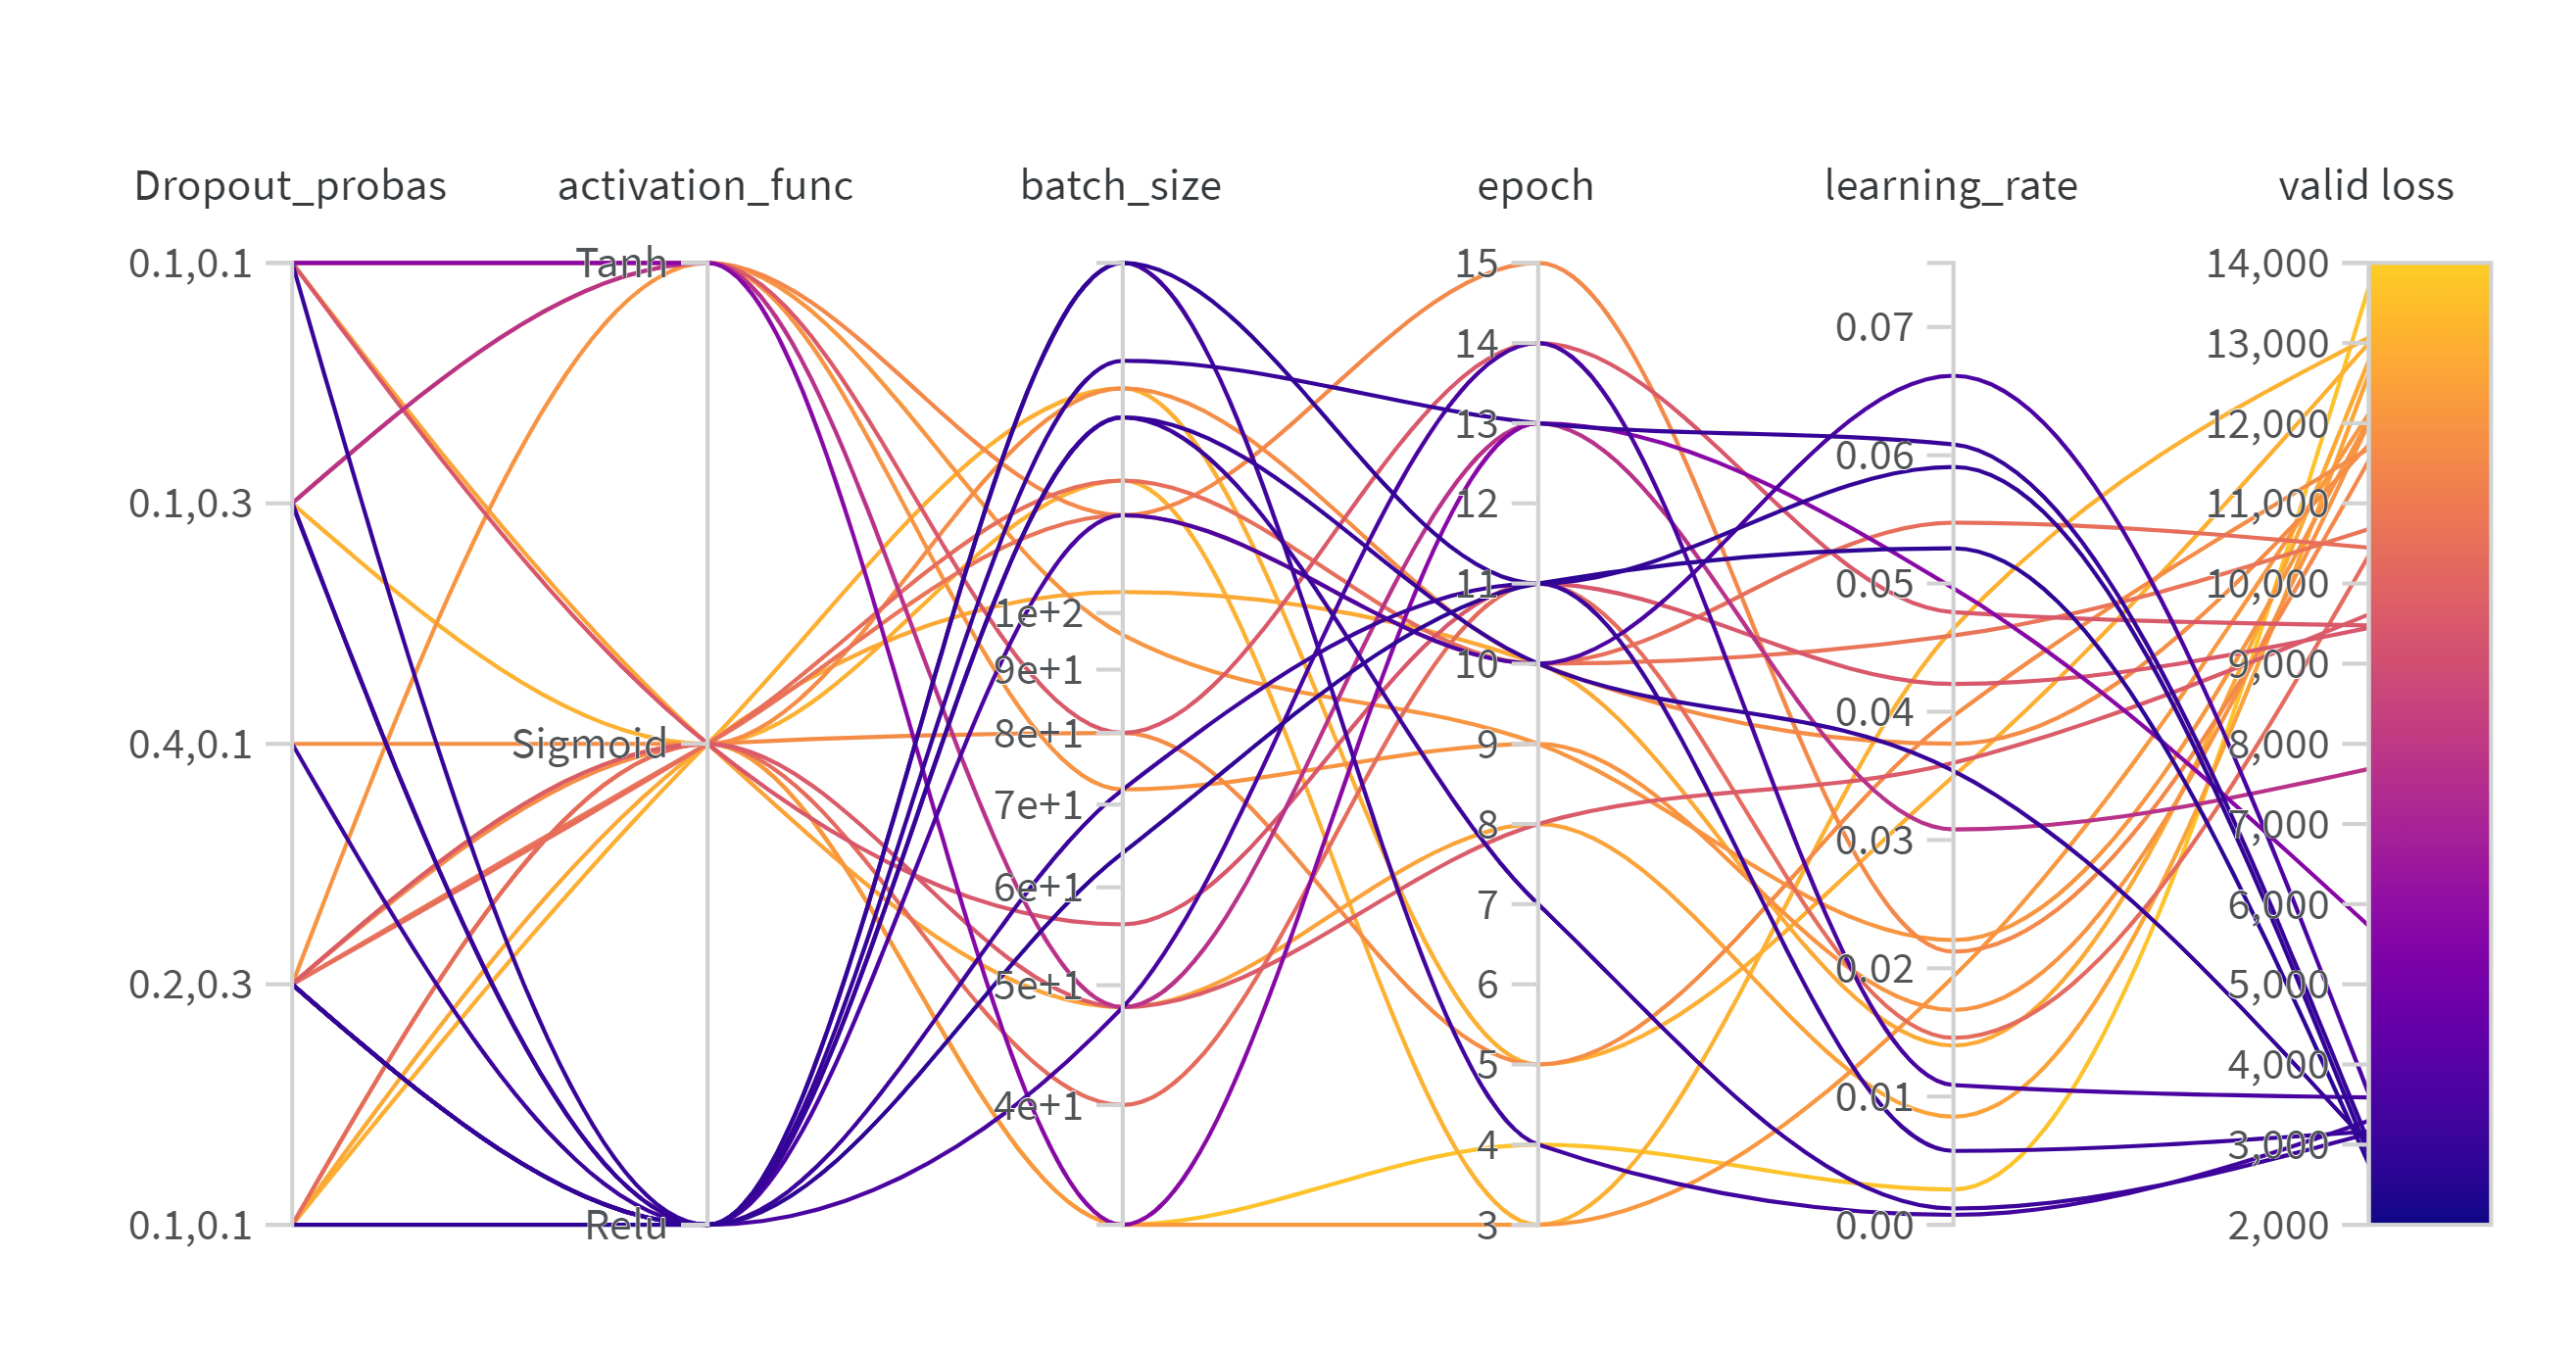
\includegraphics[width=1\textwidth]{wandbrun_1.png}
    \caption{Hyper parameters tuning results}
    \label{table:Hyper parameters tuning results MLP}
\end{figure}
\FloatBarrier

\noindent The Figure~\ref{table:Hyper parameters tuning results MLP} displays the result of \textit{Wandb} run. For thirty possible combinations of parameters drawn with our setting, we trained and evaluated the neural network with two different set of data (train and valid). Then, \textit{Wandb} shows the validation loss of each model with their respective parameter combinations. The path colour tends to a darker purple when the model had a low loss with the validation set, and to a clear yellow when it increases.
Thanks to this plot, it is straight to see that the models with a \textit{Relu} activation function tend to have pretty nice validation losses compared to the other functions.
We then decided to take the set of parameters with the lower validation loss to test our model with an other dataset. 

\FloatBarrier
\begin{table}[h]
    \centering
    \caption{Parameters selected after 30 runs}
    \label{table:Parameters of the best MLP model}

    \begin{tabular}{lrrrrrrr}
    \toprule
          Parameter & Value \\
    \midrule
    Batch Size & 64\\
    Learning Rate & 0.05274\\
    Epoch & 9\\
    Activation Function & Relu \\
    Number of Input Features & 33 \\
    Total Number of Layers & 5 \\
    Sizes of Each Layer & 30, 25, 20, 10 \\
    Dropout probabilities & 0.1, 0.1, 0.1, 0.1 \\
    \bottomrule
    \end{tabular}
\end{table}
\FloatBarrier

\noindent The Table~\ref{table:Parameters of the best MLP model} stores the parameters of the model which had the lowest validation loss after the \textit{Wandb} runs. It is important to precise that the \textit{Epoch} has been chosen during the cross validation of the model, once the other parameters were tuned. We then have 33 input features which is also so size of the first layer (one node per feature). The main improve we could make at this point would be to swap the number of layers and their sizes. Those taken here were chosen in the way to reduce the size through each layers, but those aren't optimal as we didn't swap them to test the efficiency with other possible sets. We decided to keep those parameters fixed because of the complexity of the code. 

\noindent After having find our best parameters, we tested the model by predicting prices with the test set. We ended up with a RMSE of 2688.81 with the test dataset, but we found out that the train loss (3912) was higher than both validation (2685) and test loss.

\noindent Our assumption is that our model struggled to learn and the result might be random. However we searched some reasons that could lead to this difference. 
The first one is that as we didn't tune the number of layers and their sizes, our model isn't optimal and then cannot learn efficiently. The second is that as we are using the RMSE with the ADAM optmizer to train the model, it is not appropriated. We then tried to make it learn with the MSE as a loss metric, but the results were almost similar. 
The last one is the regularization method, it can happen that the test RMSE is lower than the train because of the dropout probabilities, but here the difference is pretty high.
To check this hypothesis we trained and tested the model without dropping probabilities. 
Comparing both Figure~\ref{Training and Validation Loss with dropout probabilities} and Figure~\ref{Training and Validation Loss without dropout probabilities}, we can see that while droping with a certain probabilities some linear transformations, our model were not actually learning and that the results of the validation set prediction were random and not improving. Then, while learning without the dropout probabilities, our model could learn much better and the training loss is not anymore always above our validation loss.
\FloatBarrier
\begin{figure}[!h]
  \centering
  \begin{subfigure}{0.4\textwidth}
    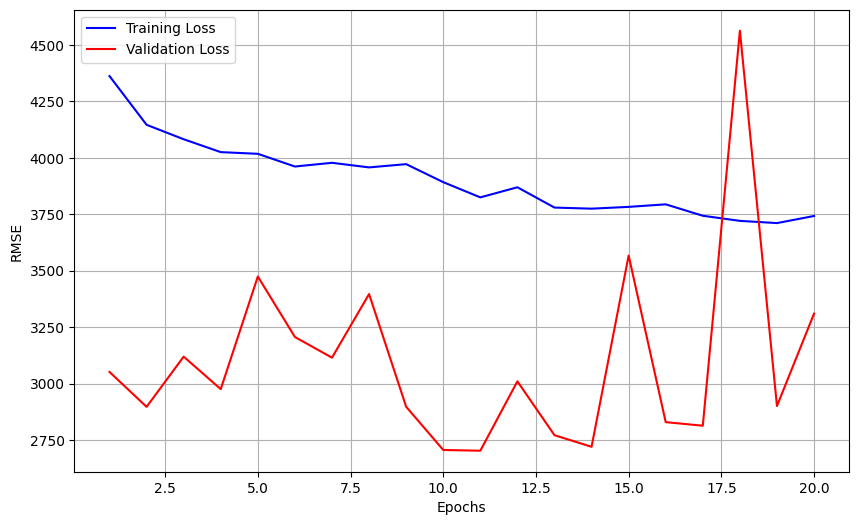
\includegraphics[width=\linewidth]{Training and Validation Loss with dropout probabilities.png}
    \caption{Training and Validation Loss with dropout probabilities}
    \label{Training and Validation Loss with dropout probabilities}
  \end{subfigure}
  \medskip
  \begin{subfigure}{0.4\textwidth}
    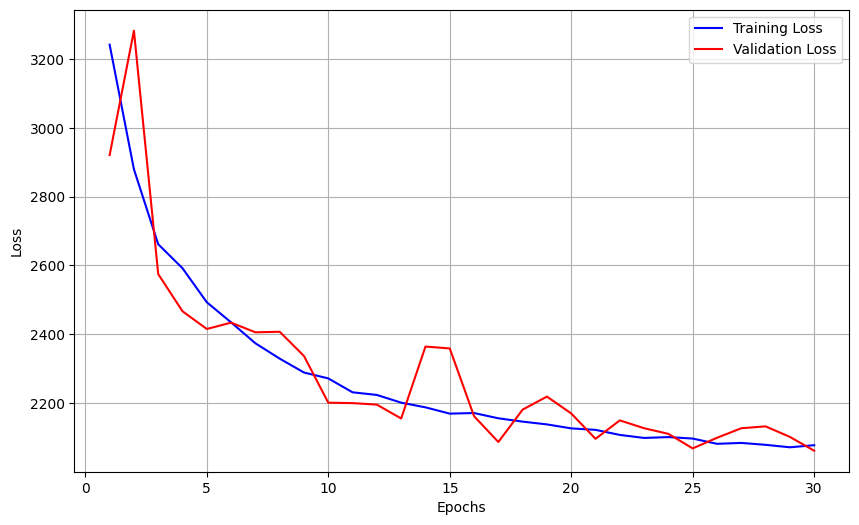
\includegraphics[width=\linewidth]{Training and Validation Loss without dropout probabilities.png}
    \caption{Training and Validation Loss without dropout probabilities}
    \label{Training and Validation Loss without dropout probabilities}
  \end{subfigure}
\end{figure}
\FloatBarrier


\noindent In the end, the Table~\ref{table:Results of the final MLP} displays the result of our final best MLP model. To make it even better, we should also try to run re-tune the hyperparameters. Unfortunately, the wandb library didn't work anymore during the last week and we didn't manage to make it run again.

\FloatBarrier
\begin{table}[h]
    \centering
    \caption{Results of the best MLP model}
    \label{table:Results of the final MLP}

    \begin{tabular}{lrrrrrrr}
    \toprule
           & RMSE \\
    \midrule
    \textbf{Train} & 2077.84\\
    \textbf{Validation} & 2061.79\\
    \textbf{Test} & 2057.50\\
    \bottomrule
    \end{tabular}
\end{table}
\FloatBarrier

\noindent \textbf{Shapley values}\\
To interpret and open the black box of the MLP model, we computed the shapley values. Having a look at the Figure~\ref{shap MLP}, we can see that the three first variables have strong and precise effect on the predicted output. It turns out that \textit{Runned\_Miles} has a negative effect on the predicted price, which is not surprising. Then, both following features have interesting effects. 
The \textit{Average\_mpg} has a low positive effect to the predicted price when it is high. But we can see that for some observations, it has a strong negative impact to the predicted output. The less miles the car can travel without any stop, the cheaper the predicted output is. This might be due to small cars which have lower engines and then lower autonomy.
It is also interesting to see that the \textit{Gas\_emission} feature does not have a clear impact on price for the lower values, but has both positive and negative impact on the price when its value is high. This suggests that the model is capturing a nuanced effect where high \textit{Gas\_emission} can be associated with both high-priced vehicles, such as sports or luxury cars, and lower-priced vehicles, potentially older cars
with less efficient engines. The presence of both positive and negative impacts at high levels of \textit{Gas\_emission} could be reflective of a diverse set of vehicles within the dataset that have high emissions for different reasons, affecting the model's price predictions in varying directions.
\FloatBarrier
\begin{figure}[ht]
    \centering
    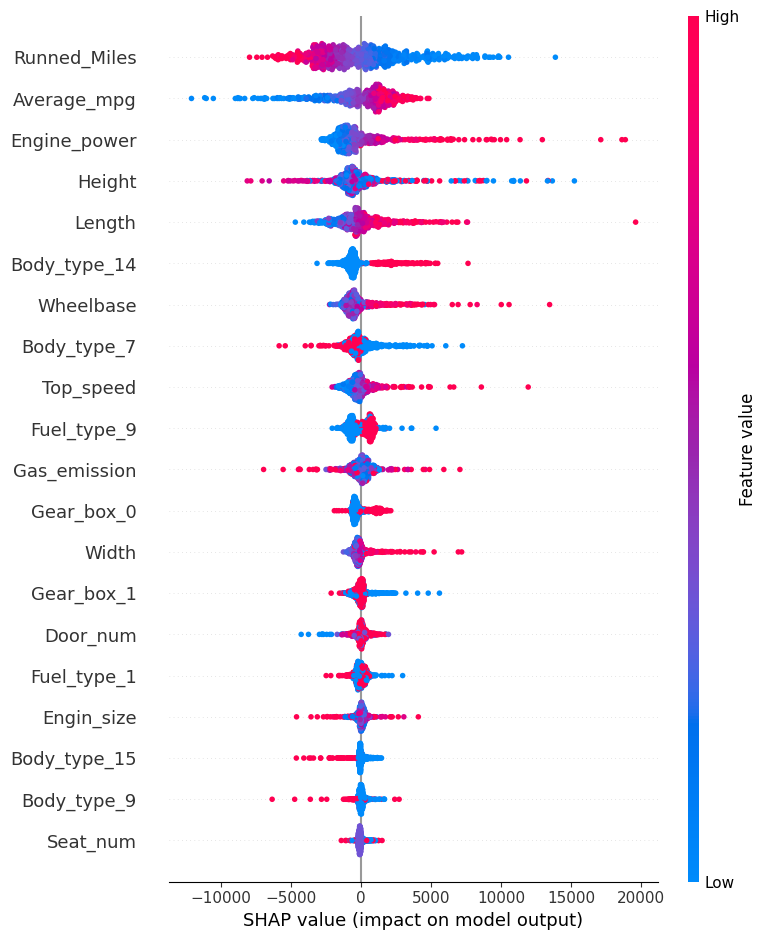
\includegraphics[width=0.5\textwidth]{shap MLP.png}
    \caption{Shapley values graph of MLP predictions}
    \label{shap MLP}
\end{figure}
\FloatBarrier


\newpage
\subsubsection{Model Comparison}

\noindent In conclusion, the Table~\ref{Model_comparison} summarizes the results achieved by each model using the categorical and nummerical data. The most performant model was the XGBoost model with a RMSE of 1418.60 on the test set. However, every models that used a reduction method were slightly less performant, such as the KNN with 11 PCA components with a RMSE score of 1735.86 on the validation set, compared to 1719.35 on the KNN without reduction. The least effective model was the Multi-Layer Perceptron when trained on reduced data.\\
These results indicate that models performed comparably when reduction methods were applied, which can be useful for a potential benefit in terms of computational efficiency.

\FloatBarrier
\begin{table}[h!]
    \centering
    \caption{Model comparison}

    \begin{tabular}{lccc}
        \toprule
        \textbf{Model} & \multicolumn{2}{c}{\textbf{RMSE}} \\
        \cmidrule{2-3}
         & \textbf{Training} & \textbf{Test} \\
        \midrule
        \textbf{KNN} & 1254.05 & 1719.35 \\
        \textbf{KNN + PCA} & 1272.46 & 1735.86 \\
        \textbf{XGBOOST} & \textbf{1178.93} & \textbf{1418.60} \\
        \textbf{XGBOOST + Elastic Net} & 1185.53 & 1443.99 \\
        \textbf{MLP} & 2077.84 & 2057.50 \\
        \textbf{MLP + PCA} & 2983.15 & 3056.08 \\
        \bottomrule
    \end{tabular}
    \label{Model_comparison}
\end{table}
\FloatBarrier
\noindent \\
\noindent Comparing the shapley values computed for the XGBoost (Figure~\ref{xgboostshapley}) and MLP (Figure~\ref{shap MLP}) models we can notice some difference in the ranges of feature effects. Those are due to the data used for the shapley computations. For the MLP, only a batch of data were used while for XGBoost, all of the data. Otherwise, it's interesting to see that the effects are globally the same and only importance rank differs.

\subsection{Predictive Analysis: Car price prediction with image data}
 
\noindent \textbf{Hyper-parameter optimization} \\
\noindent Optimizing any model is a crucial step and in the case of the pre-trained ResNet18 model, we swapped two hyperparameters: the \textit{learning rate} and the \textit{batch size}. Indeed, the Resnet18 algorithm is based on the stochastic descent gradient, its convergence will highly depends on these hyperparameters. While a large batch size facilitates computational efficiency and results in smoother convergence, a smaller batch size is preferred to generalize to unseen data.\\

\noindent The \textit{learning rate} determines the size of the step during the optimization. If the learning rate is too high we can miss the convergence because the step size are too big and with a low learning rate we can obtain a local minima and not the global one. Hence, it is really important to test different values to find the best one.


\FloatBarrier
\begin{table}[h]
    \centering
    \caption{Hyperparameters tested of Resnet18}
    \begin{tabular}{lrrrrrrr}
    \toprule
           & Minimum & Maximum & Distribution \\
    \midrule
     Learning rate & 0.0005 & 0.07 & Uniform  \\
     Batch size & 30 & 200 & Q\_log\_Uniform  \\
    \bottomrule
     \label{hyperparameters test CNN}
    \end{tabular}
\end{table} \\ [0.1 cm]
\FloatBarrier

\noindent The table~\ref{hyperparameters test CNN} is the summary table of the range of the batch size and the learning rate that we wanted to test. As the Resnet-18 model was pre-trained, we kept the trained weights and re-trained them with our data for the price prediction task.

\FloatBarrier
\begin{figure}[ht]
    \centering
    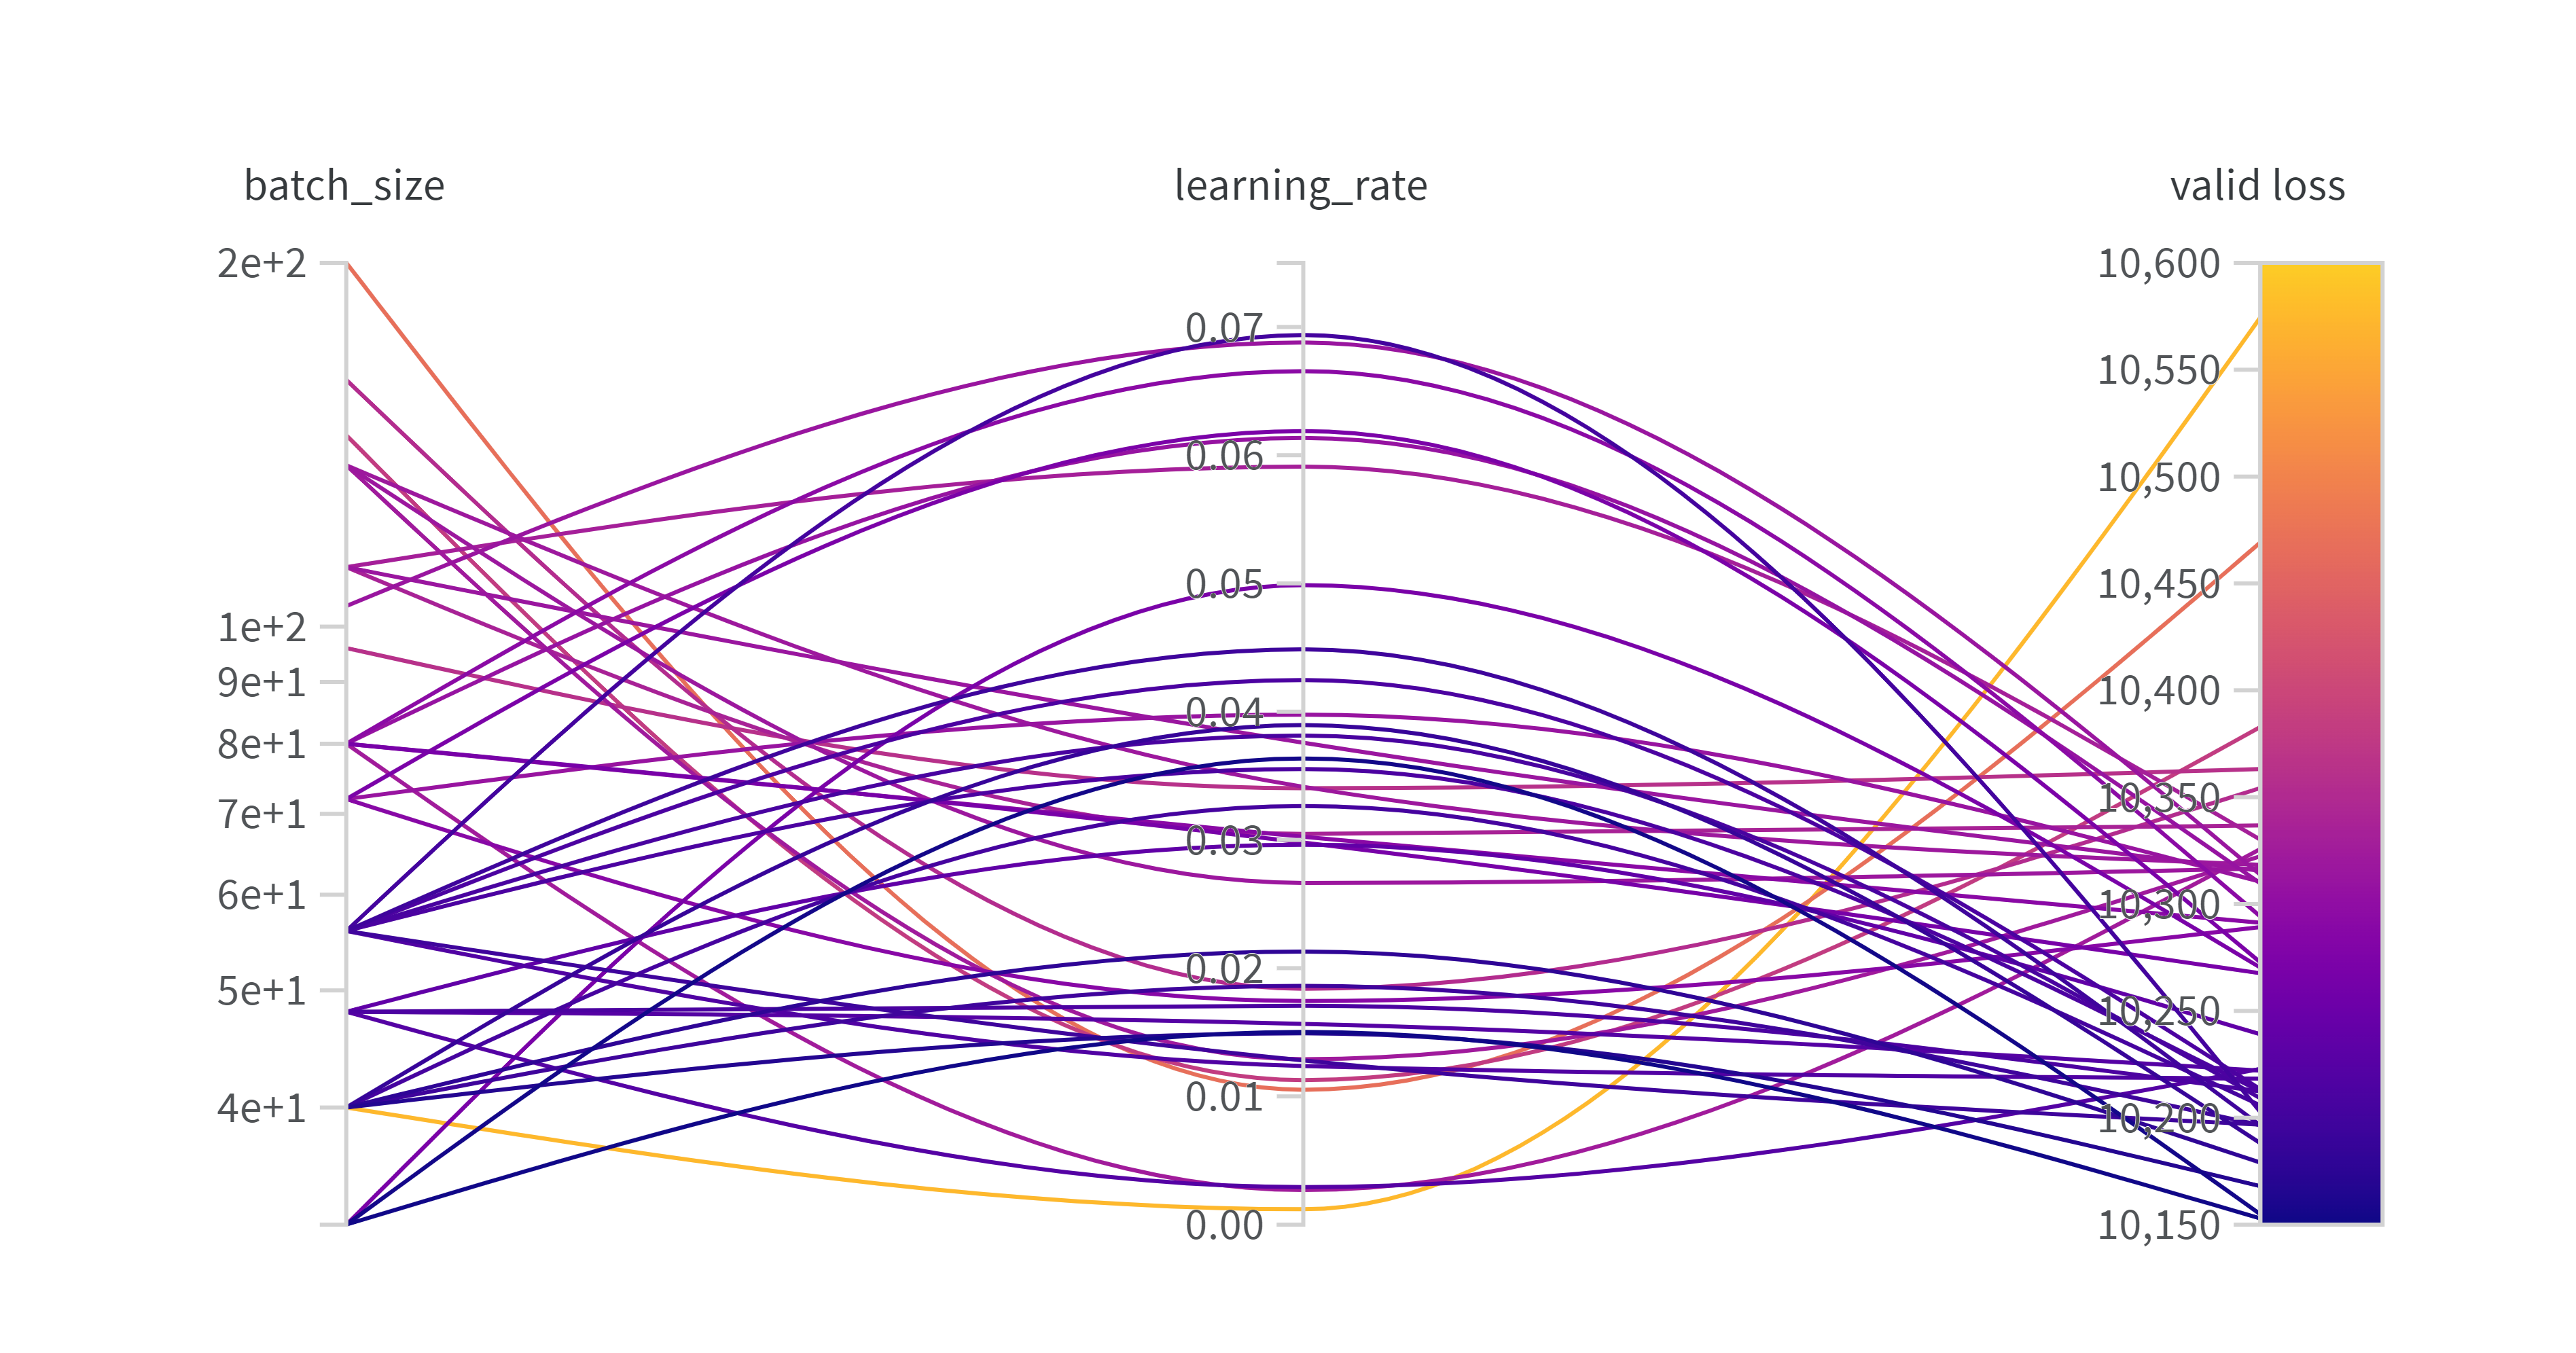
\includegraphics[width=0.7\textwidth]{cnn_wandb.png}
    \caption{Hyper parameters tuning results for the Resnet18}
    \label{Tuning CNN}
\end{figure}
\FloatBarrier

\noindent The Figure~\ref{Tuning CNN} shows the result of the hyperparameters optimization with Wandb. We tested around 40 possible combinations for the possible values of the batch size and the learning rate. As explained before, the color depends on the score of the loss. As we wanted the lowest valid loss to select the optimal hyperparameter we took the bluest path. Each run was made for 3 epochs. As the model was pre-trained, it did  not take long to converge to the lowest loss possible. 


\noindent \textbf{Best model selected} \\
\noindent After determining the best parameters with the validation set, we tested our model on the test set and analysed the results. As we wanted to be sure that two or three epochs would be enough, we trained the model with 6 epochs. We see in the Figure~\ref{Training CNN} that the training loss decreases from 17000 to a bit lower than 16000 with the first update of the weights. Then, until the last epochs, there is no improvement in the loss.


\noindent 
\FloatBarrier
\begin{figure}[ht]
    \centering
    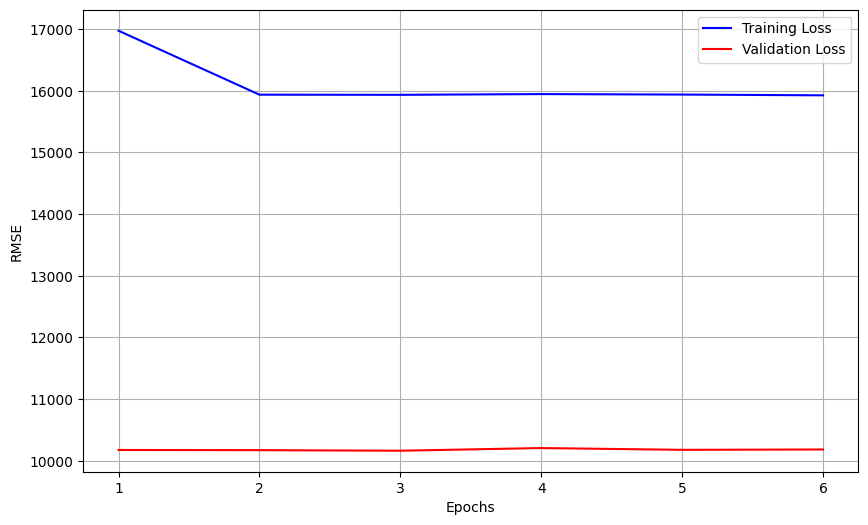
\includegraphics[width=0.5\textwidth]{training CNN.png}
    \caption{training CNN}
    \label{Training CNN}
\end{figure}
\FloatBarrier



\FloatBarrier
\begin{table}[h]
    \centering
    \caption{Hyperparameters selected for Resnet18}
    \label{Hyperparameters Resnet18}
    \begin{tabular}{lrrrrrrr}
    \toprule
    Hyperparameter & Value \\
    \midrule
     Learning rate & 0.01503 \\
     Batch size & 32\\
    \bottomrule
    \end{tabular}
\end{table} \\ [0.1 cm]
\FloatBarrier

\noindent The Table~\ref{Hyperparameters Resnet18} shows the values selected for the hyper-parameters. The learning rate is pretty small and can be due to the pre-trained weights, which doesn't need much more to changed. A small update after the first epoch is enough.

\FloatBarrier
\begin{table}[h]
    \centering
    \caption{Results of the Resnet18 model}
    \label{Results CNN}
    \begin{tabular}{lrrrrrrr}
    \toprule
           & RMSE \\
    \midrule
    Train & 15945.92\\
    Validation & 10176.11\\
    Test & 10746.46\\
    \bottomrule
    \end{tabular}
\end{table}
\FloatBarrier




\noindent The Table~\ref{Results CNN} displays the results of the CNN model on the different sets. We obtained an RMSE close to that of the validation test, which is 30\% lower than that in the training set. This can be explained by the data normalization and data augmentation that we did to prepare as effectively as possible the inputs for the pre-trained model. As the data were not rotated for the evaluation and testing set, it is easier for the model to predict the price and have a lower loss than with the training set. Unfortunately, we cannot compare this result with the ones from the categorical and numerical data because the original dataset was not the same. 


\section{Conclusion}
Following the recommendations for further research of previous studies on car price prediction, this elaboration applied and compared some promising machine learning algorithms to the CAR-DVM dataset from \cite{chen2017comparative}. After explaining our model selection and introducing the used model-agnostic as well as information reduction methods, we applied these methods to numerical, categorical and image data. We have found that the XGBoost model provided the best performance with a RMSE value of 1418.60. These findings are in line with previous studies such as \cite{Pudaruth2014} and \cite{Gajera2021} who also suggest that more complex machine learning models provide better car price predictions. Surprisingly however, the XGBoost outperfomed the MLP model which showed an RMSE of 2057.50. With a deeper optimisation of hyperparameters, we could improve the MLP performance. By keeping the ReLU activation and removing dropout probabilities, we could find for the other parameters some optimal region and reducing their swapping range values.\\

\noindent Furthermore, we could observe that applying different information reduction methods did not improve but indeed worsen the performance of our models. One explanation is the fact that some models such as the XGBoost automatically account for model complexity and variable selection by construction. Comparing the shapley values generated for the XGBoost and MLP, we can observe some similarities. Both algorithms heavily rely on the features runned miles (mileage), engine power, body type 14 and Length. In contrast, the MLP accounts more importance to some further variables such as height or wheelbase to make its predictions. \\

\noindent Putting our results into the perspective of previous studies like \cite{Gajera2021} or \cite{Karakoç2020}, we must note that applying machine learning models to \textit{larger} data did not lead to a significant model performance as expected. Technically seen an RMSE of 1418.60 and accuracy greater than 97\% represents a very good model fit. In practice however differences in car valuations of \$1418.60 might not be accurate enough for merchants and car resellers. To account for that, a possible strategy could be to optimize specific models for certain car price ranges which might be a limitation of our models.\\

\noindent Even though comparing model performance in terms of RMSE might be misleading, e.g. due to differences in the data, we did not manage to obtain model performances similar to \cite{yang2018ai} when using only image data for car price prediction. That said, for the CNN model, we could have also fit other pre-trained models to our data. Using deeper models such as Resnet50 or Resnet101 and comparing their results could be subject to further research but requires better computation capacities. Moreover, with more resources allocated to the coding, we could have managed to fit the CNN with the same dataset as the MLP and therefore do the concatenation.

 \newpage
 \printbibliography
 

\end{document}
